%! Author = ThinkPad Pro
%! Date = 15/10/2025

% Preamble
\documentclass[11pt]{article}

% Packages
\usepackage{amsmath}

% Document

\usepackage[utf8]{inputenc}
\usepackage[english]{babel}

\usepackage{amsfonts}
\usepackage{amssymb}
\usepackage{graphicx}
\usepackage{hyperref}
\usepackage[numbers,sort&compress]{natbib}
\usepackage{booktabs}
\usepackage{float}
\usepackage{subcaption}
\usepackage{geometry}
\usepackage{fancyhdr}
\usepackage{setspace}
\usepackage{titlesec}
\usepackage{listings}
\usepackage{xcolor}

% Page geometry
\geometry{left=2.5cm,right=2.5cm,top=3cm,bottom=3cm}

% Header and footer
\pagestyle{fancy}
\fancyhf{}
\fancyhead[L]{EEG Dataset Analysis - BCI Competition IV 2a}
\fancyhead[R]{\thepage}
\renewcommand{\headrulewidth}{0.4pt}

% Line spacing
\onehalfspacing

% Section formatting
\titleformat{\section}{\Large\bfseries}{\thesection}{1em}{}
\titleformat{\subsection}{\large\bfseries}{\thesubsection}{1em}{}
\titleformat{\subsubsection}{\normalsize\bfseries}{\thesubsubsection}{1em}{}

% Code listing style
\lstset{
    backgroundcolor=\color{gray!10},
    basicstyle=\ttfamily\small,
    breaklines=true,
    captionpos=b,
    commentstyle=\color{green!50!black},
    frame=single,
    keywordstyle=\color{blue},
    language=Python,
    numbers=left,
    numberstyle=\tiny\color{gray},
    showstringspaces=false,
    stringstyle=\color{red},
    tabsize=2
}

\title{\textbf{EEG Dataset Analysis Report: \\ BCI Competition IV Dataset 2a \\ Motor Imagery Classification}}
\author{Rahma Aroua \\ Supervised by: Dr. Tiehang Duan}
\date{\today}
\setlength{\headheight}{14pt}

\begin{document}
\maketitle
\newpage

\begin{abstract}
This report presents a comprehensive analysis of the BCI Competition IV Dataset 2a, focusing on motor imagery classification using electroencephalography (EEG) signals. We developed a complete pipeline encompassing data exploration, signal preprocessing, feature extraction, and classification. The methodology includes bandpass filtering (8-30 Hz), Independent Component Analysis for artifact removal, Common Spatial Patterns for feature extraction, and evaluation of multiple machine learning classifiers. Our best model, Random Forest, achieved 67.66\% accuracy (Cohen's Kappa = 0.57) on four-class motor imagery tasks, demonstrating the feasibility of non-invasive brain-computer interfaces for distinguishing left hand, right hand, feet, and tongue movements. All code and analyses are available in a reproducible GitHub repository.
\end{abstract}

\newpage
\tableofcontents
\newpage

\section{Introduction}

Brain-Computer Interfaces (BCIs) represent a transformative technology enabling direct communication between the human brain and external devices, bypassing conventional neuromuscular pathways \citep{wolpaw2000brain}. This capability holds profound implications for individuals with motor impairments, offering potential pathways to restore communication and control.

This study focuses on motor imagery-based BCIs, where users mentally rehearse movements without physical execution \citep{pfurtscheller1999motor}. Motor imagery activates similar cortical regions as actual movement, producing measurable patterns in electroencephalography (EEG) signals that can be decoded into control commands.

\subsection{Research Objectives}

The primary objectives of this study are:

\begin{enumerate}
    \item Develop a robust preprocessing pipeline for EEG motor imagery data
    \item Extract discriminative features capturing neural correlates of motor imagery
    \item Implement and compare multiple classification approaches
    \item Validate results using rigorous cross-validation and statistical testing
    \item Create a reproducible analysis framework for BCI research
\end{enumerate}

\subsection{Dataset: BCI Competition IV 2a}

We analyze the BCI Competition IV Dataset 2a \citep{brunner2008bci}, a standardized benchmark for motor imagery classification. The dataset includes:

\begin{itemize}
    \item \textbf{Participants:} 9 healthy subjects (A01-A09)
    \item \textbf{Tasks:} Four motor imagery classes (left hand, right hand, feet, tongue)
    \item \textbf{Recording:} 22 EEG channels (10-20 system) + 3 EOG channels
    \item \textbf{Sampling Rate:} 250 Hz
    \item \textbf{Trials:} 288 per session (72 per class)
\end{itemize}

This dataset provides a challenging four-class problem requiring sophisticated signal processing and feature extraction to achieve accurate classification.

\section{Theoretical Background}

\subsection{Motor Imagery and Neurophysiology}

Motor imagery involves mentally simulating movements without physical execution \citep{pfurtscheller1999motor}. Neuroimaging studies reveal that motor imagery activates similar cortical areas as actual movement, including the primary motor cortex, supplementary motor area, and premotor cortex.

\subsubsection{Event-Related Desynchronization (ERD)}

During motor imagery, power decreases in the mu (8-12 Hz) and beta (13-30 Hz) frequency bands occur over the motor cortex contralateral to the imagined movement \citep{pfurtscheller1999motor}. This phenomenon, called Event-Related Desynchronization (ERD), reflects increased cortical activation and serves as a primary feature for motor imagery classification.

\subsubsection{Event-Related Synchronization (ERS)}

Following motor imagery, power often rebounds above baseline levels in the beta band, termed Event-Related Synchronization (ERS). This rebound indicates cortical inhibition and task disengagement.

\subsection{Common Spatial Patterns (CSP)}

Common Spatial Patterns is a supervised spatial filtering technique that maximizes variance for one class while minimizing it for another \citep{ramoser2000optimal}. For two classes with covariance matrices $C_1$ and $C_2$, CSP solves the generalized eigenvalue problem:

\begin{equation}
C_1 W = \lambda (C_1 + C_2) W
\end{equation}

The spatial filters $W$ are ordered by eigenvalues $\lambda$, where extreme values indicate high discriminability. For multi-class problems, we employ a One-Versus-Rest approach, computing CSP filters for each class against all others.

\section{Methodology}

\subsection{Data Exploration and Validation}

Initial data exploration verified dataset integrity and signal quality using MNE-Python \citep{gramfort2013meg}. We examined:

\begin{itemize}
    \item Channel amplitudes and distributions
    \item Class balance across motor imagery tasks
    \item Frequency characteristics via Power Spectral Density
    \item Electrode positioning and spatial coverage
\end{itemize}

\begin{figure}[H]
    \centering
    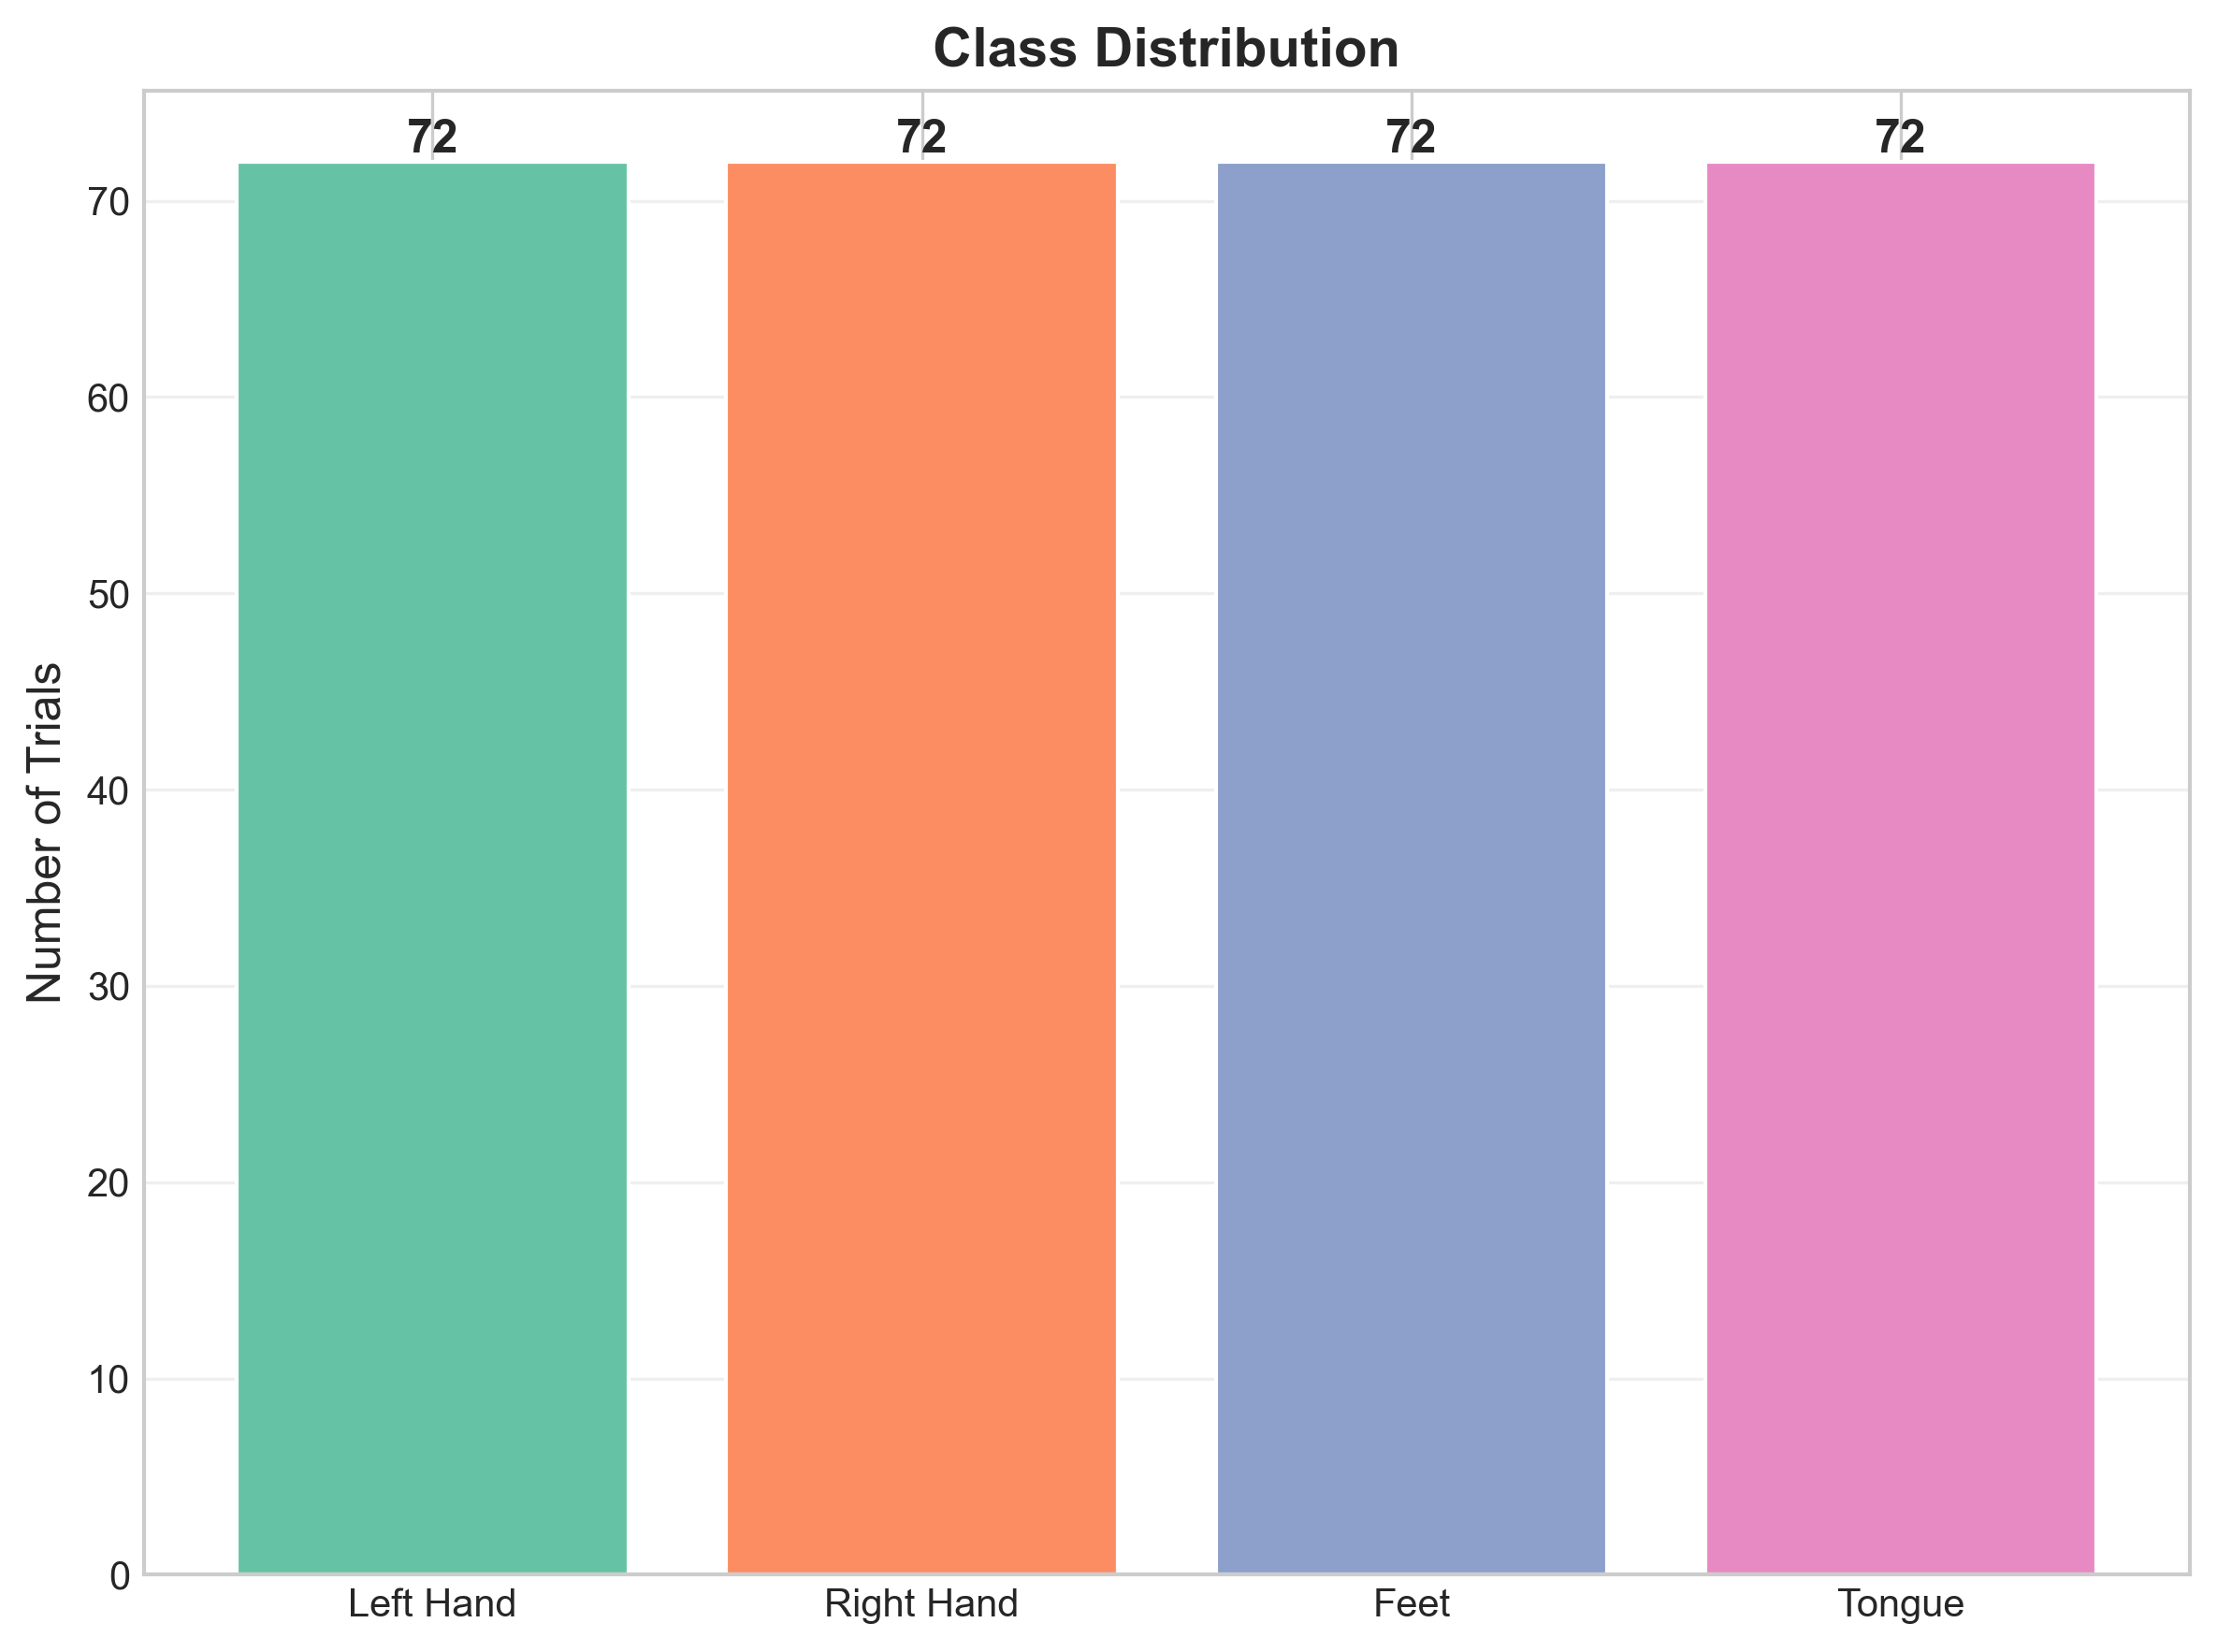
\includegraphics[width=0.7\textwidth]{../results/figures/01_class_distribution.png}
    \caption{Class distribution showing perfect balance with 72 trials per motor imagery task (Subject A01T).}
    \label{fig:class_distribution}
\end{figure}

Figure~\ref{fig:class_distribution} confirms balanced representation across all four motor imagery classes, ensuring unbiased model training. Mean EEG amplitudes across channels ranged from 12-43 $\mu$V, consistent with typical EEG recordings and indicating good signal quality.

\subsection{Preprocessing Pipeline}

A comprehensive preprocessing pipeline was implemented to enhance signal quality and remove artifacts \citep{gramfort2013meg,delorme2004eeglab}:

\subsubsection{Bandpass Filtering (8-30 Hz)}

A Butterworth bandpass filter isolated sensorimotor rhythms relevant for motor imagery \citep{pfurtscheller1999motor}:

\begin{itemize}
    \item \textbf{Mu band (8-12 Hz):} Primary sensorimotor rhythm
    \item \textbf{Beta band (13-30 Hz):} Motor-related activity
\end{itemize}

\subsubsection{Notch Filtering (50 Hz)}

Power line interference at 50 Hz was removed using a notch filter to eliminate electrical noise.

\subsubsection{Independent Component Analysis (ICA)}

ICA decomposed EEG signals into independent components \citep{hyvarinen2000independent,delorme2004eeglab}, enabling identification and removal of artifacts:

\begin{itemize}
    \item \textbf{Ocular artifacts:} Eye blinks and movements
    \item \textbf{Muscle artifacts:} Facial and neck muscle activity
    \item \textbf{Cardiac artifacts:} Heartbeat-related interference
\end{itemize}

\begin{figure}[H]
    \centering
    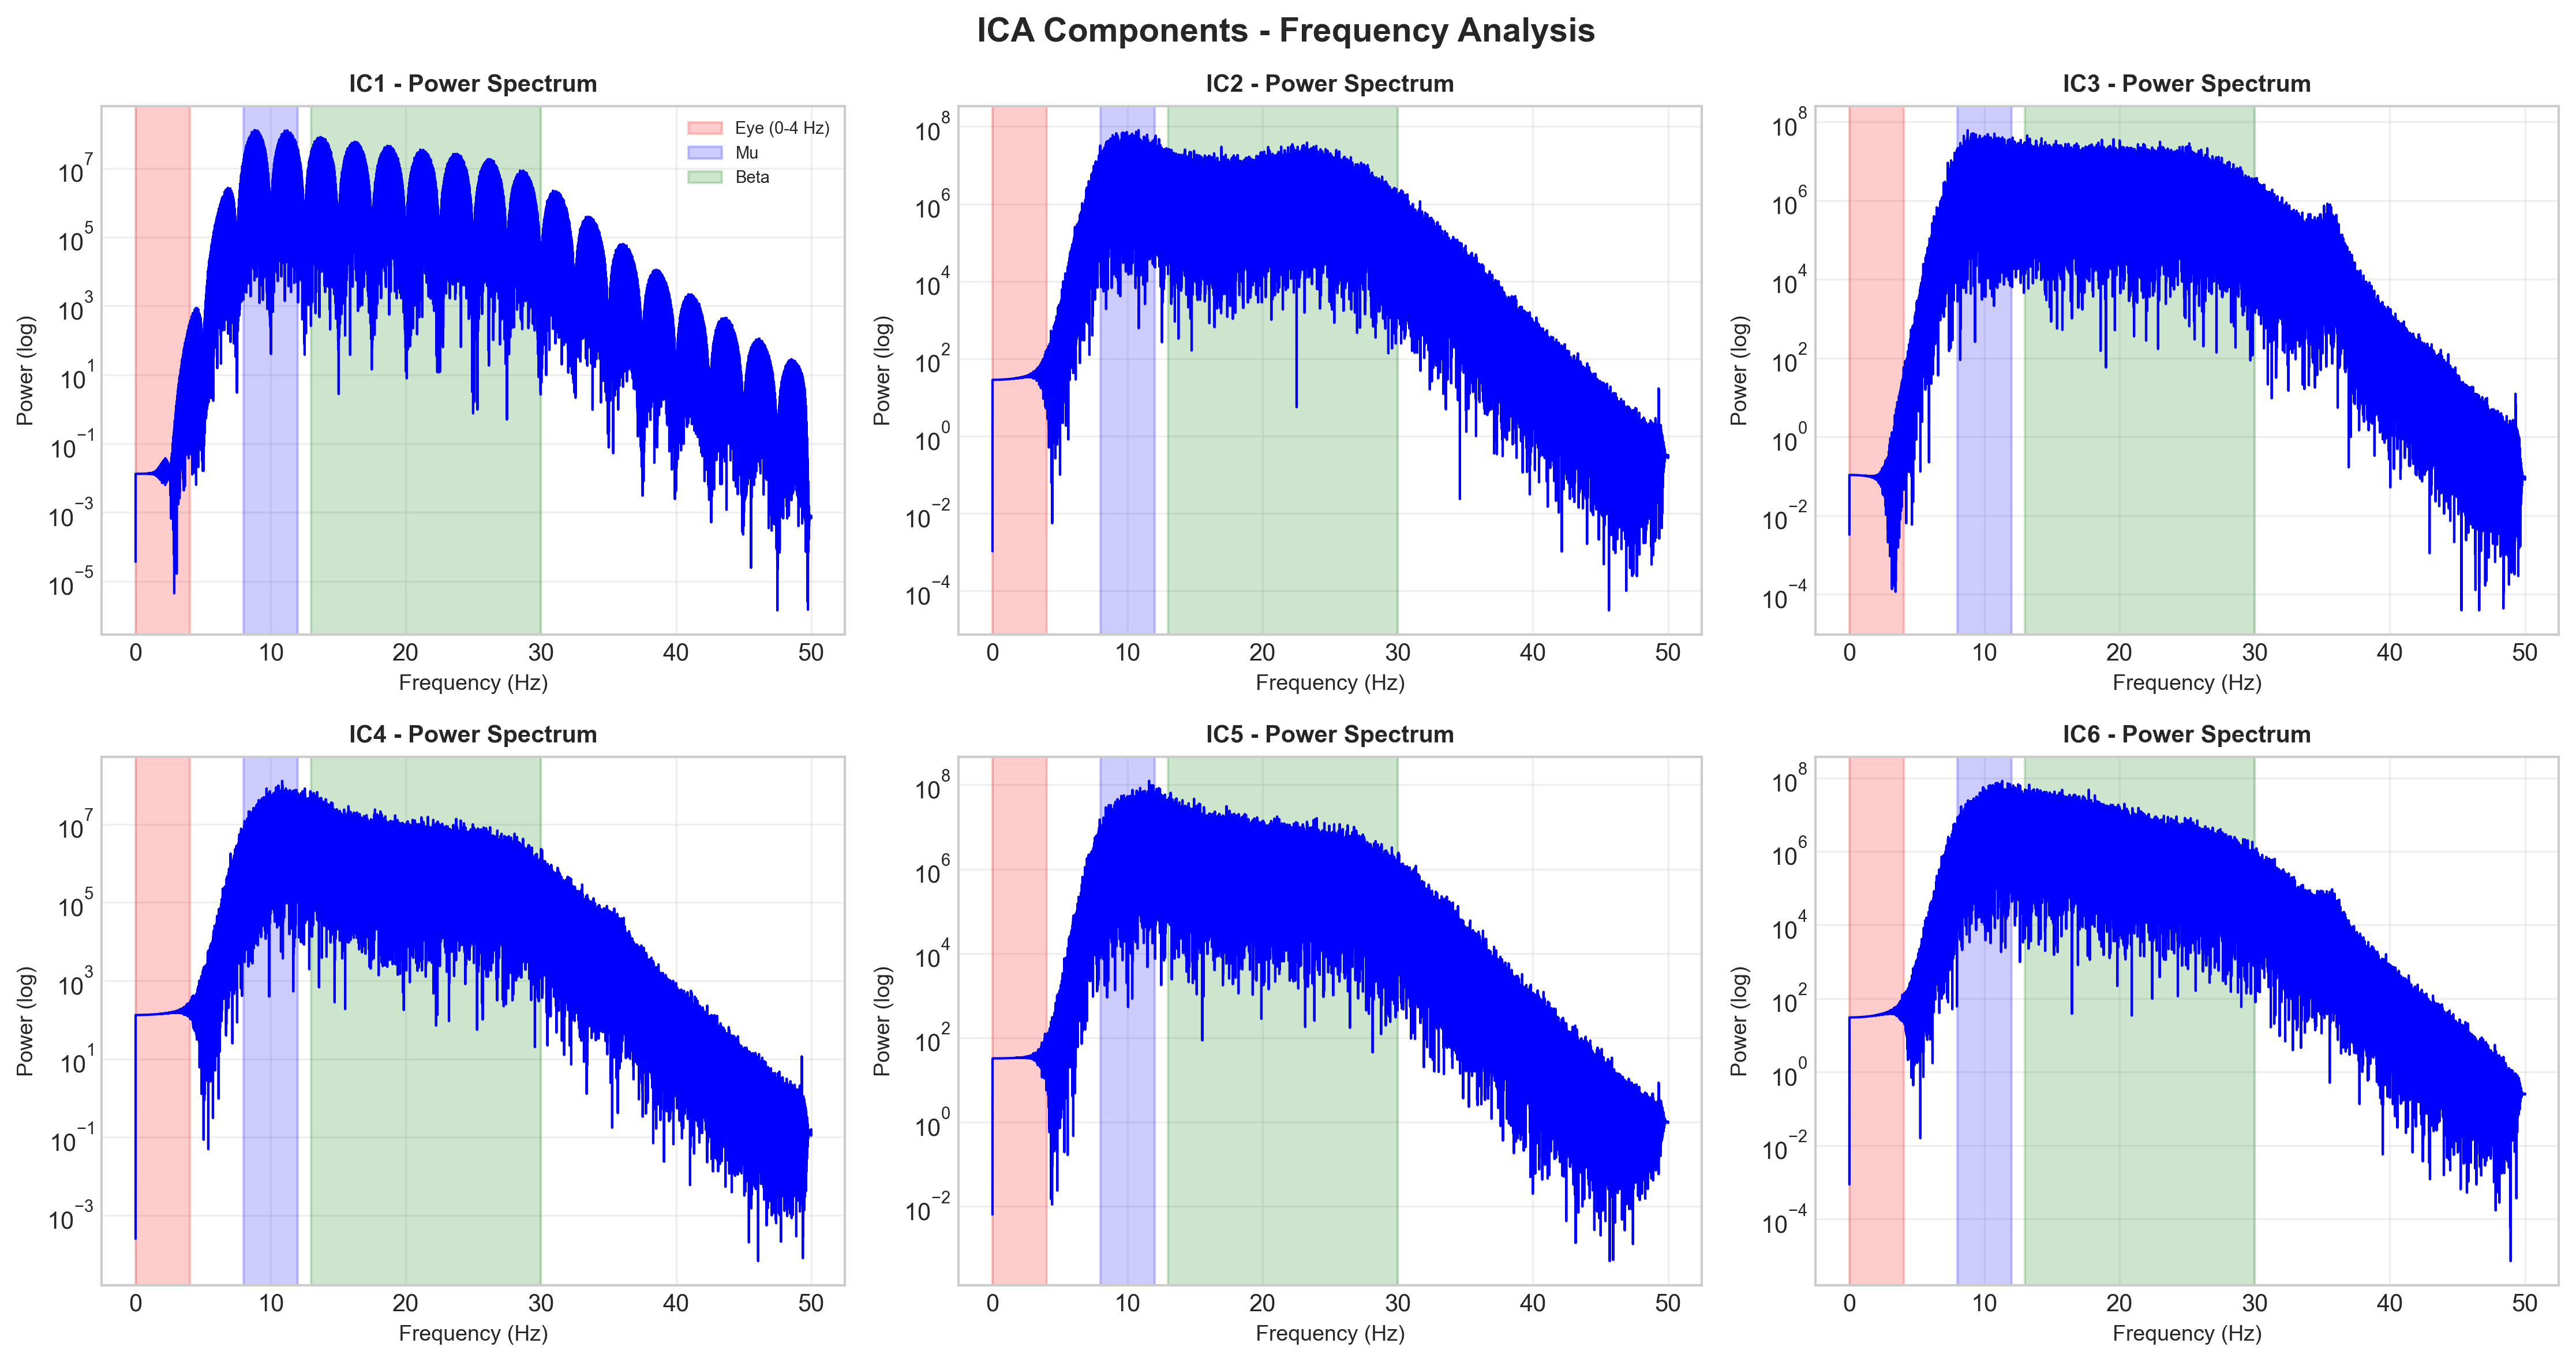
\includegraphics[width=0.85\textwidth]{../results/figures/02_ica_components_spectrum.png}
    \caption{Independent Component Analysis frequency spectra. Components with high power below 4 Hz were identified as eye movement artifacts and removed.}
    \label{fig:ica_components}
\end{figure}

Figure~\ref{fig:ica_components} illustrates ICA component frequency characteristics. Components showing dominant power in the 0-4 Hz range with high correlation to EOG channels were excluded as ocular artifacts.

\subsubsection{Common Average Reference (CAR)}

All electrodes were re-referenced to the average of all electrodes, reducing spatially correlated noise and improving signal-to-noise ratio.

\subsubsection{Epoching and Baseline Correction}

Continuous data were segmented into trials spanning -0.5 to 4.0 seconds relative to cue onset. Each trial was baseline-corrected using the pre-stimulus interval (-0.5 to 0 seconds) to normalize for pre-task activity variations.

\begin{figure}[H]
    \centering
    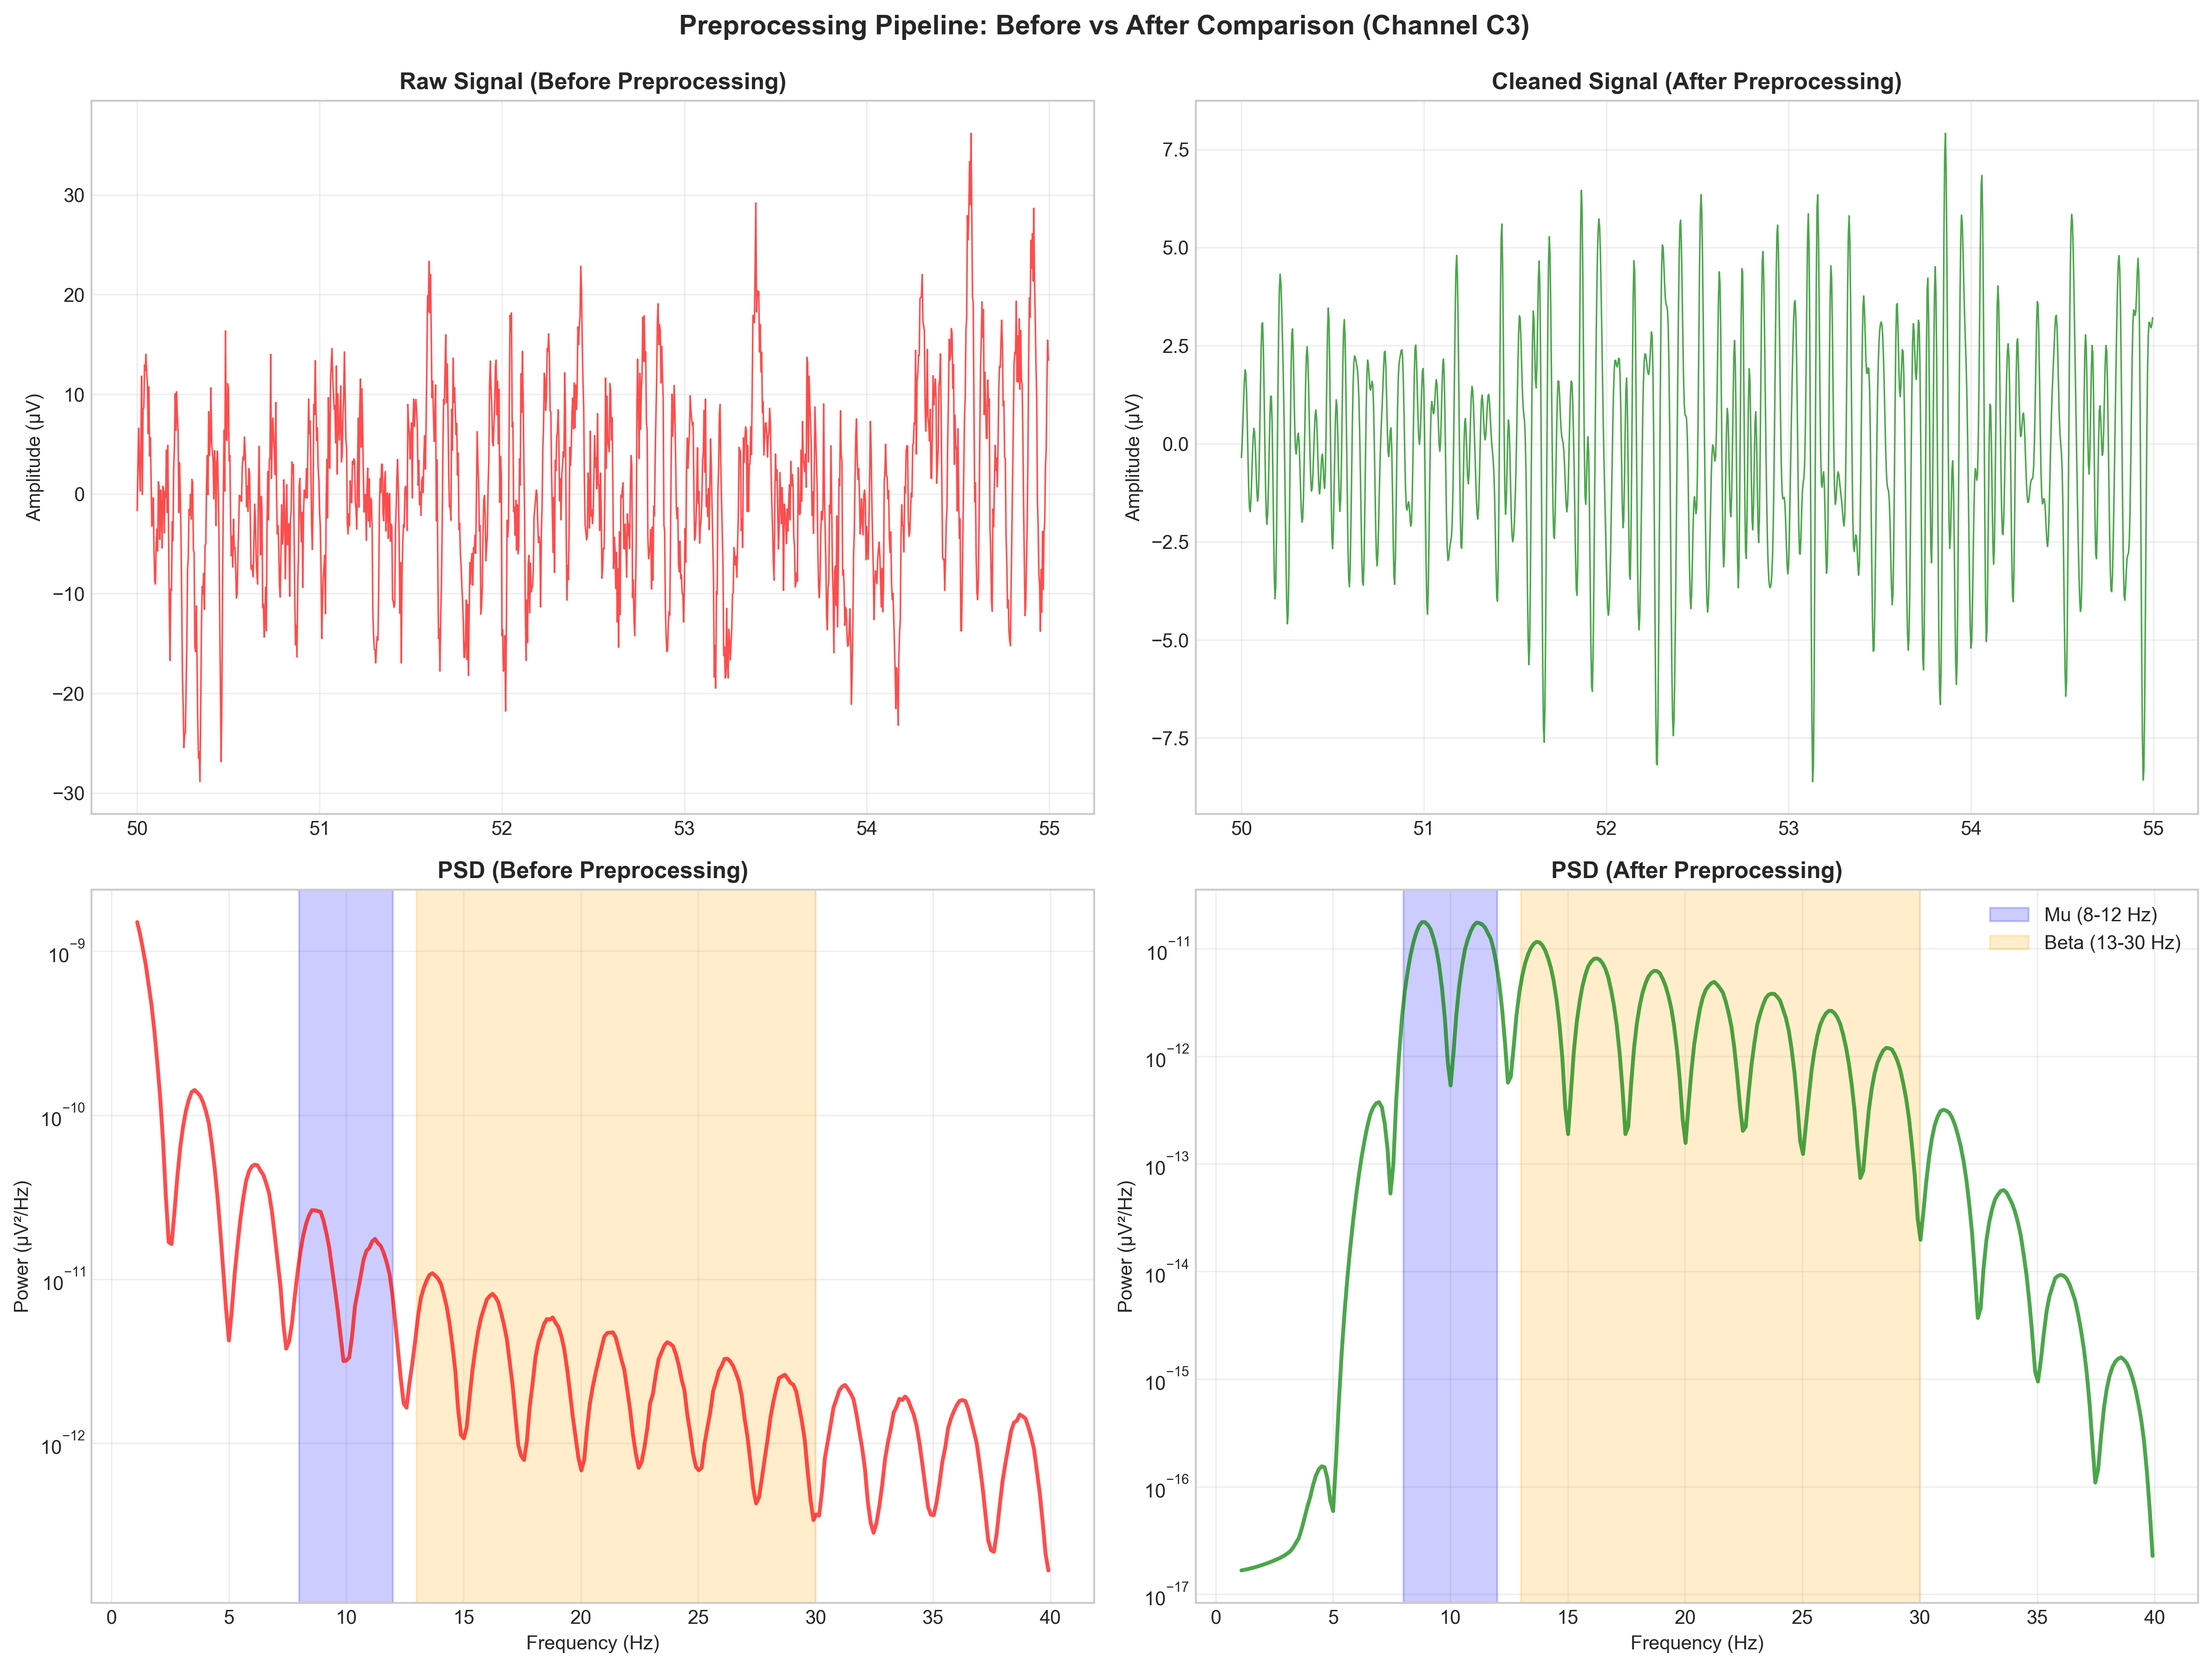
\includegraphics[width=0.95\textwidth]{../results/figures/02_comprehensive_comparison.png}
    \caption{Comprehensive before/after preprocessing comparison for channel C3, showing (top) time-domain signal quality improvement and (bottom) frequency-domain noise reduction with preserved sensorimotor rhythms.}
    \label{fig:preprocessing_comparison}
\end{figure}

Figure~\ref{fig:preprocessing_comparison} demonstrates the effectiveness of the preprocessing pipeline. The time-domain signals (top panels) show artifact removal while preserving neural oscillations. The frequency-domain analysis (bottom panels) reveals successful isolation of mu (8-12 Hz) and beta (13-30 Hz) bands with elimination of power line noise and out-of-band frequencies.

\subsection{Feature Extraction}

A comprehensive feature set was extracted to capture spatial, spectral, and temporal characteristics of motor imagery \citep{lotte2018review}:

\subsubsection{Common Spatial Patterns (CSP)}

CSP filters were computed using a One-Versus-Rest approach for the four-class problem \citep{ramoser2000optimal}. For each class, we selected the first and last 3 components (6 components total), yielding 6 CSP features per trial.

\begin{figure}[H]
    \centering
    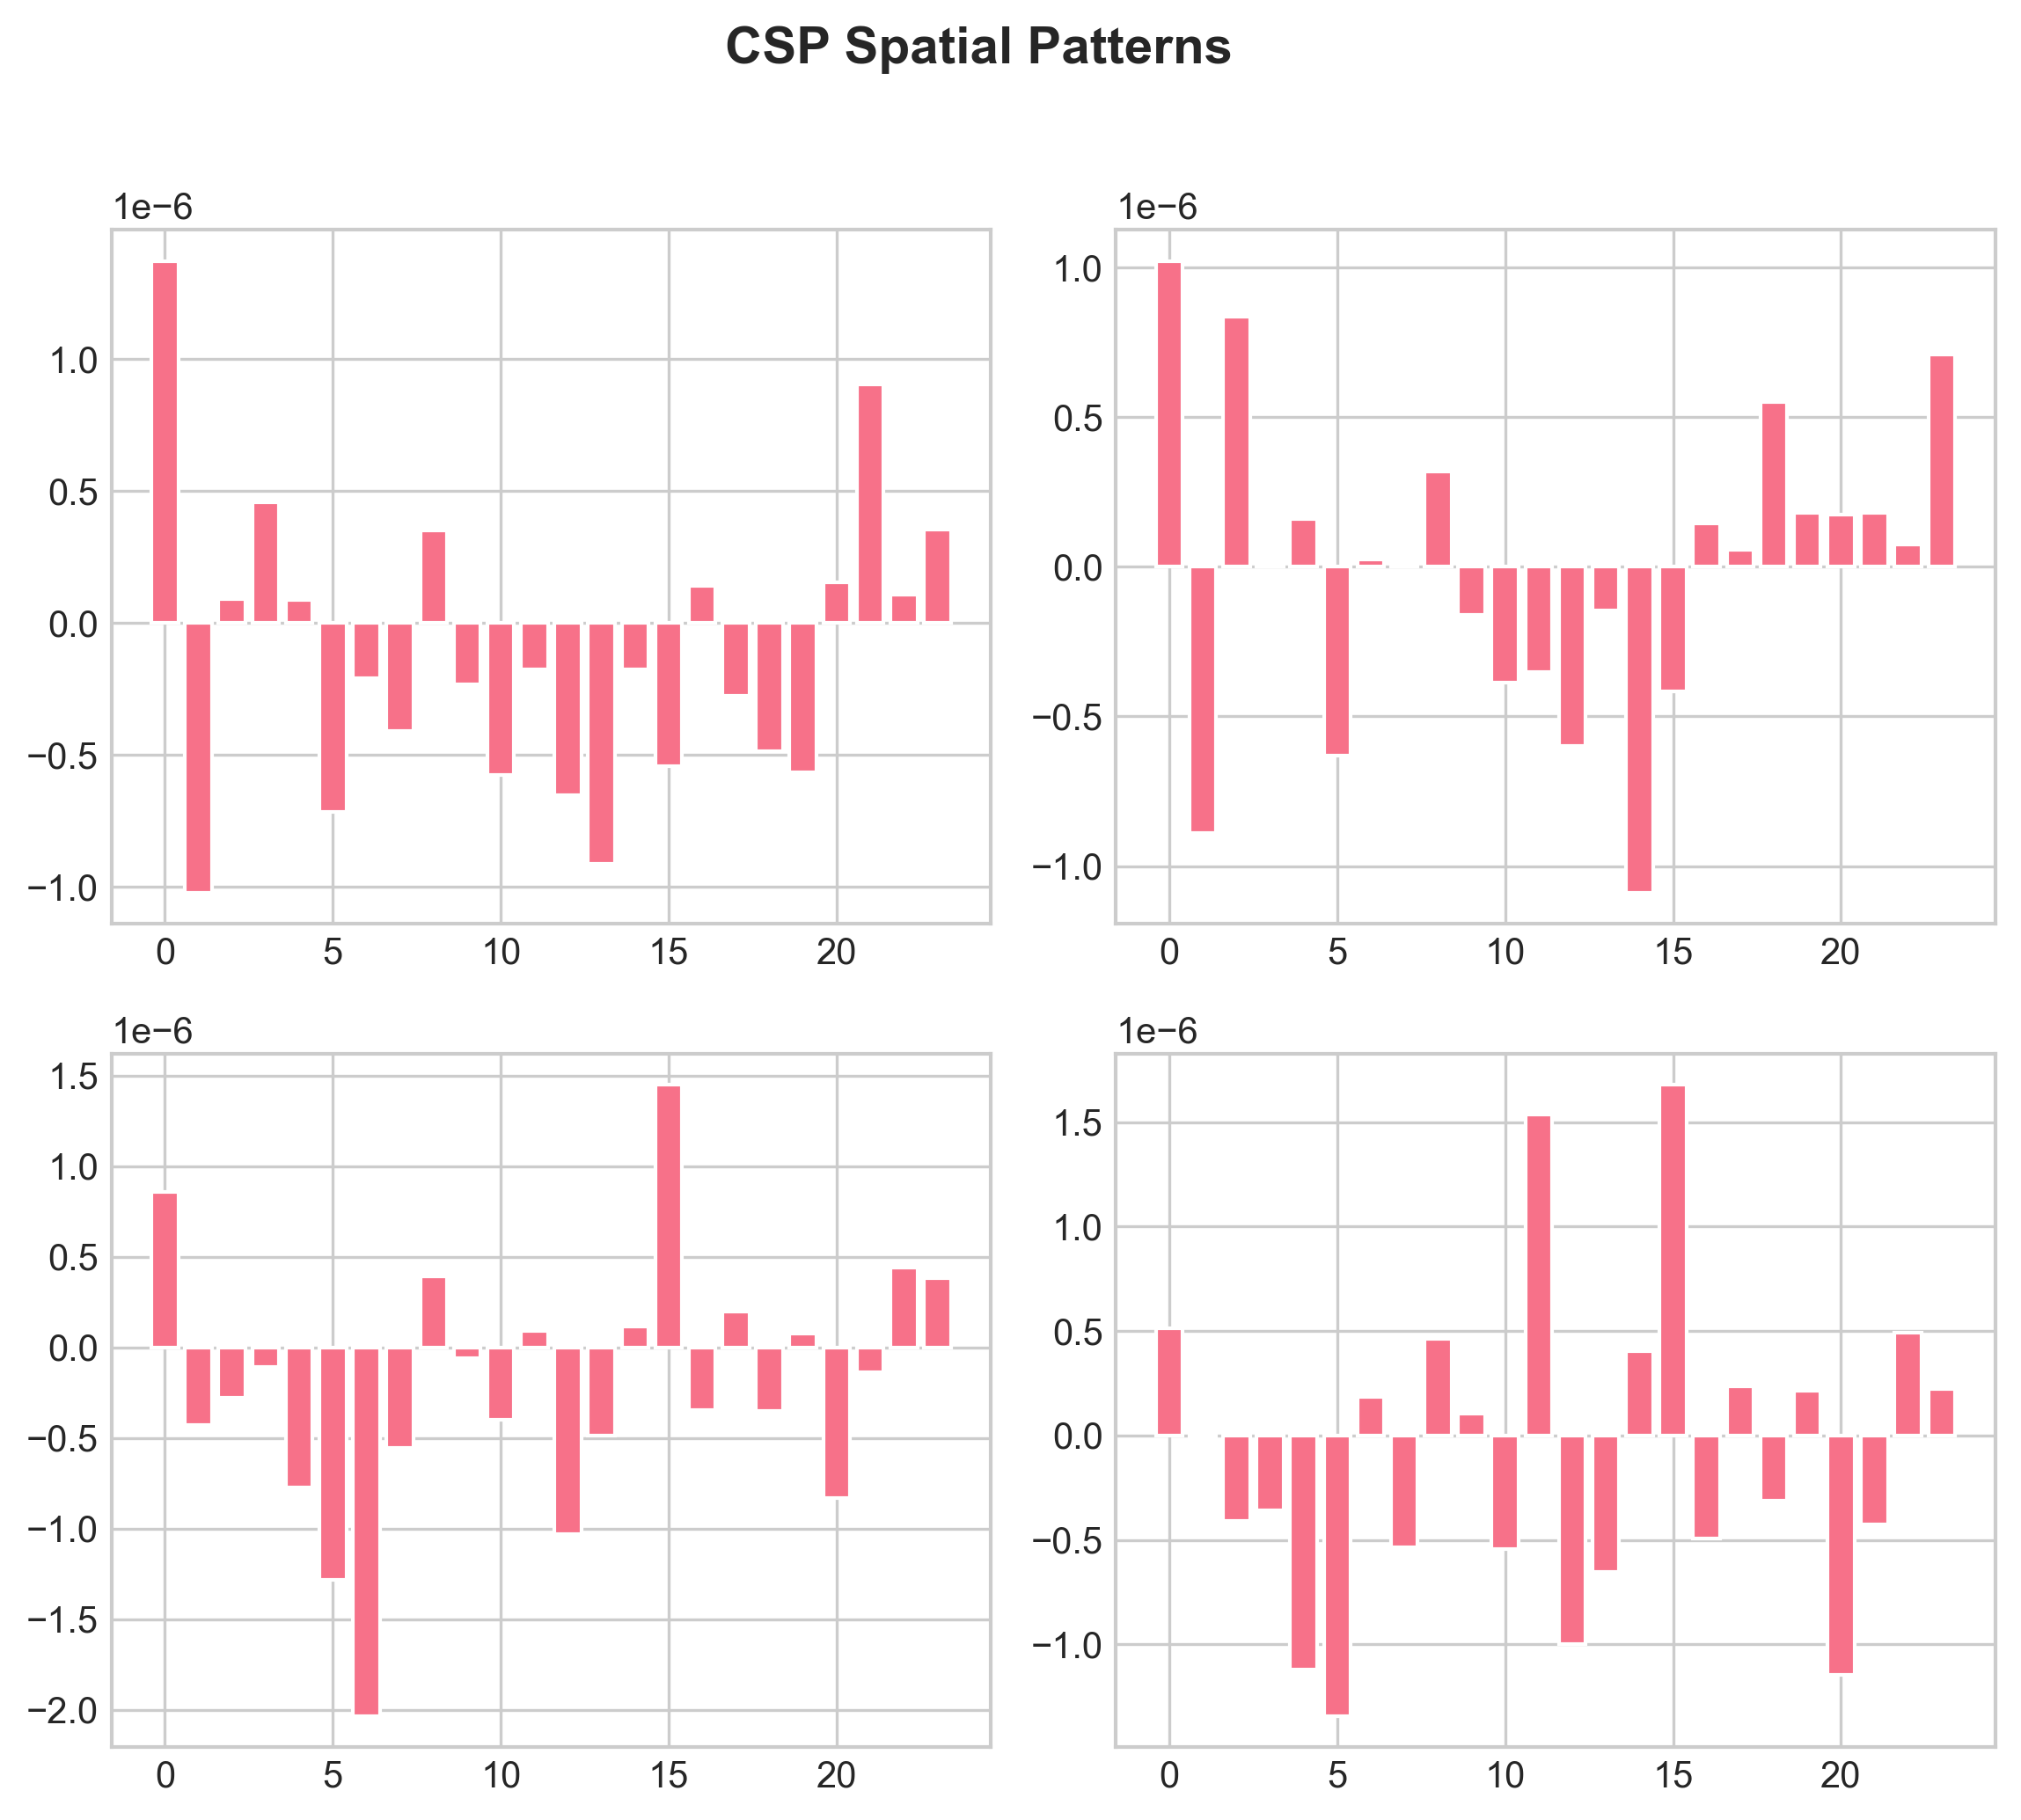
\includegraphics[width=0.95\textwidth]{../results/figures/03_csp_spatial_patterns.png}
    \caption{CSP spatial patterns for Subject A01 showing contralateral motor cortex organization. Top row: patterns emphasizing left hemisphere (right hand imagery). Bottom row: patterns emphasizing right hemisphere (left hand imagery).}
    \label{fig:csp_patterns}
\end{figure}

Figure~\ref{fig:csp_patterns} visualizes learned CSP spatial patterns. The topographic maps reveal the expected neurophysiological organization: patterns associated with right hand imagery show activation over the left motor cortex (C3 region), while left hand patterns activate the right motor cortex (C4 region). This contralateral organization validates the CSP extraction process.

\subsubsection{Spectral Features}

Band power was computed across four frequency bands using Welch's method:

\begin{itemize}
    \item Mu band (8-12 Hz)
    \item Low beta band (13-20 Hz)
    \item High beta band (20-30 Hz)
    \item Full beta band (13-30 Hz)
\end{itemize}

For 22 channels and 4 bands, this yielded 88 spectral features per trial.

\subsubsection{Hjorth Parameters}

Three time-domain descriptors were computed per channel \citep{hjorth1970eeg}:

\begin{itemize}
    \item \textbf{Activity:} Signal variance (power)
    \item \textbf{Mobility:} Mean frequency estimate
    \item \textbf{Complexity:} Bandwidth estimate
\end{itemize}

This contributed 66 features (22 channels × 3 parameters).

\subsubsection{Statistical Features}

Basic statistical measures captured amplitude distribution characteristics:

\begin{itemize}
    \item Mean amplitude
    \item Standard deviation
    \item Skewness (distribution asymmetry)
    \item Kurtosis (distribution tailedness)
\end{itemize}

This added 88 features (22 channels × 4 statistics).

The complete feature vector contained 248 features per trial (6 CSP + 88 band power + 66 Hjorth + 88 statistical).

\begin{figure}[H]
    \centering
    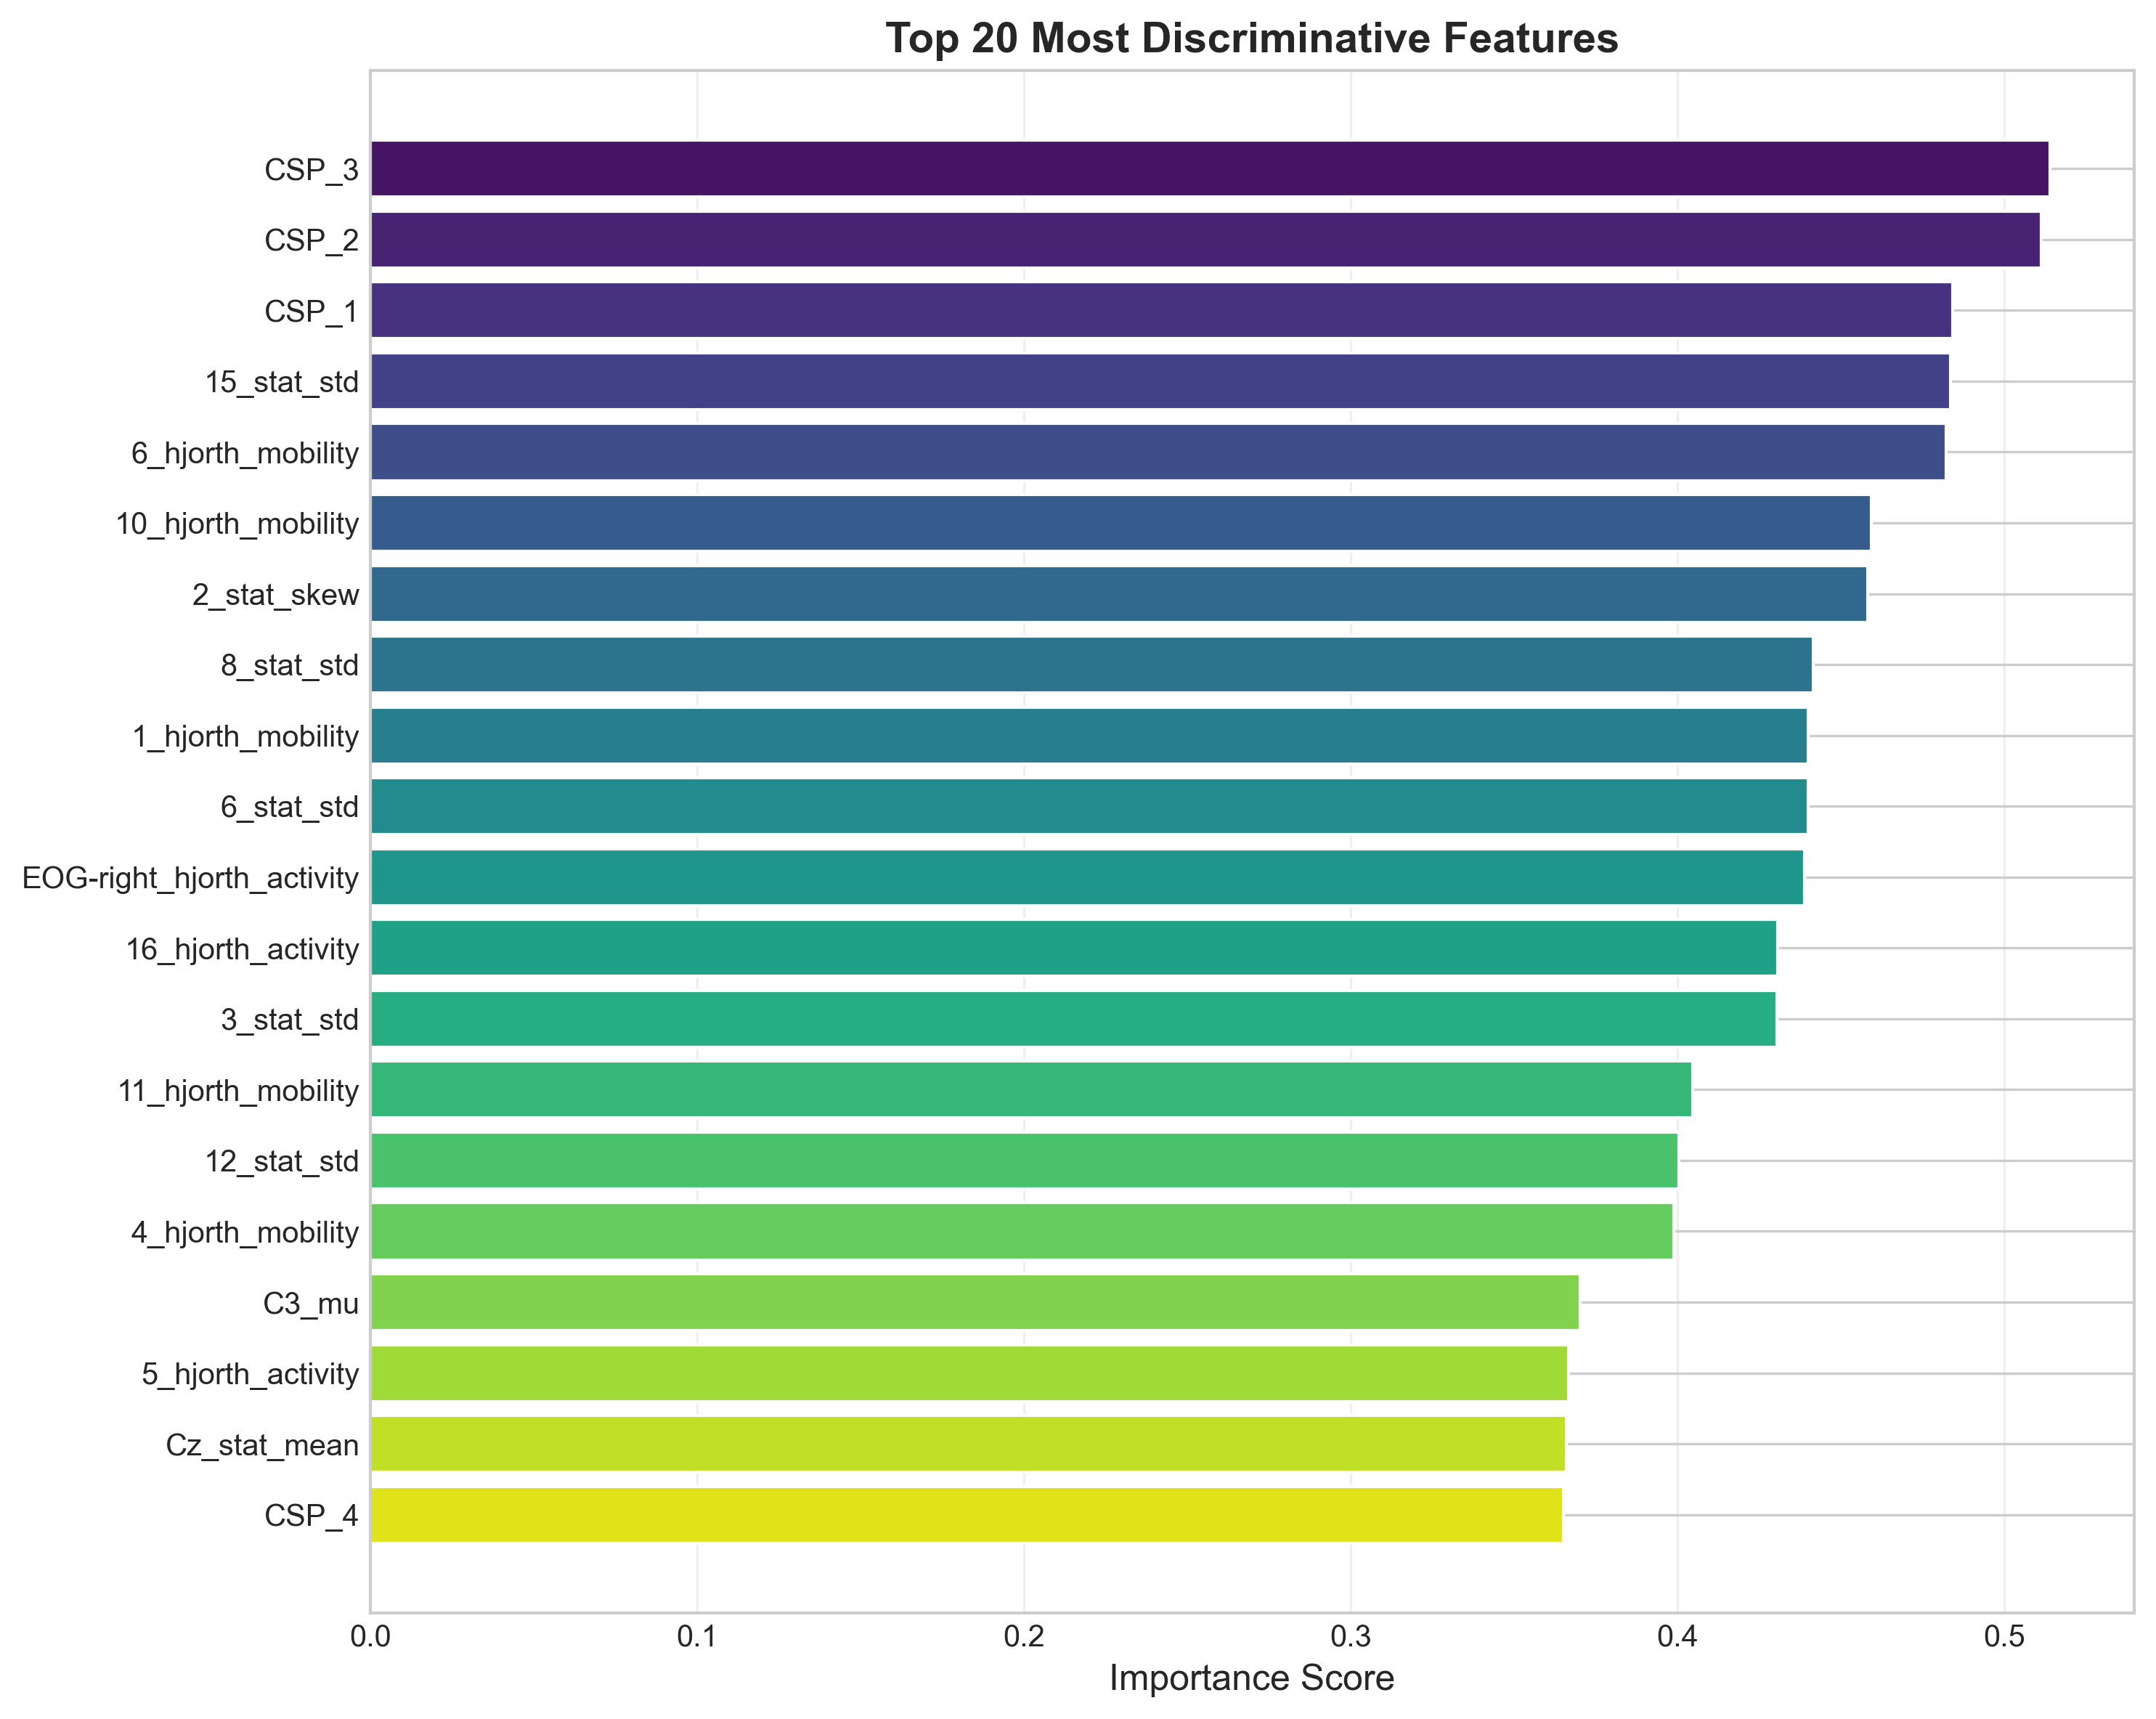
\includegraphics[width=0.85\textwidth]{../results/figures/03_feature_importance_top20.png}
    \caption{Top 20 most discriminative features ranked by mutual information with class labels. CSP components dominate, followed by mu and beta band power from central motor channels.}
    \label{fig:feature_importance}
\end{figure}

Figure~\ref{fig:feature_importance} shows feature importance analysis using mutual information. CSP features exhibit the highest discriminative power, with all 6 components ranking in the top 10. Among spectral features, mu and beta band power from central motor cortex electrodes (C3, Cz, C4) demonstrate strong class separability, confirming these frequency bands' relevance for motor imagery classification.

\subsubsection{Time-Frequency Analysis}

Event-Related Desynchronization/Synchronization (ERD/ERS) patterns were visualized to validate neurophysiological plausibility:

\begin{figure}[H]
    \centering
    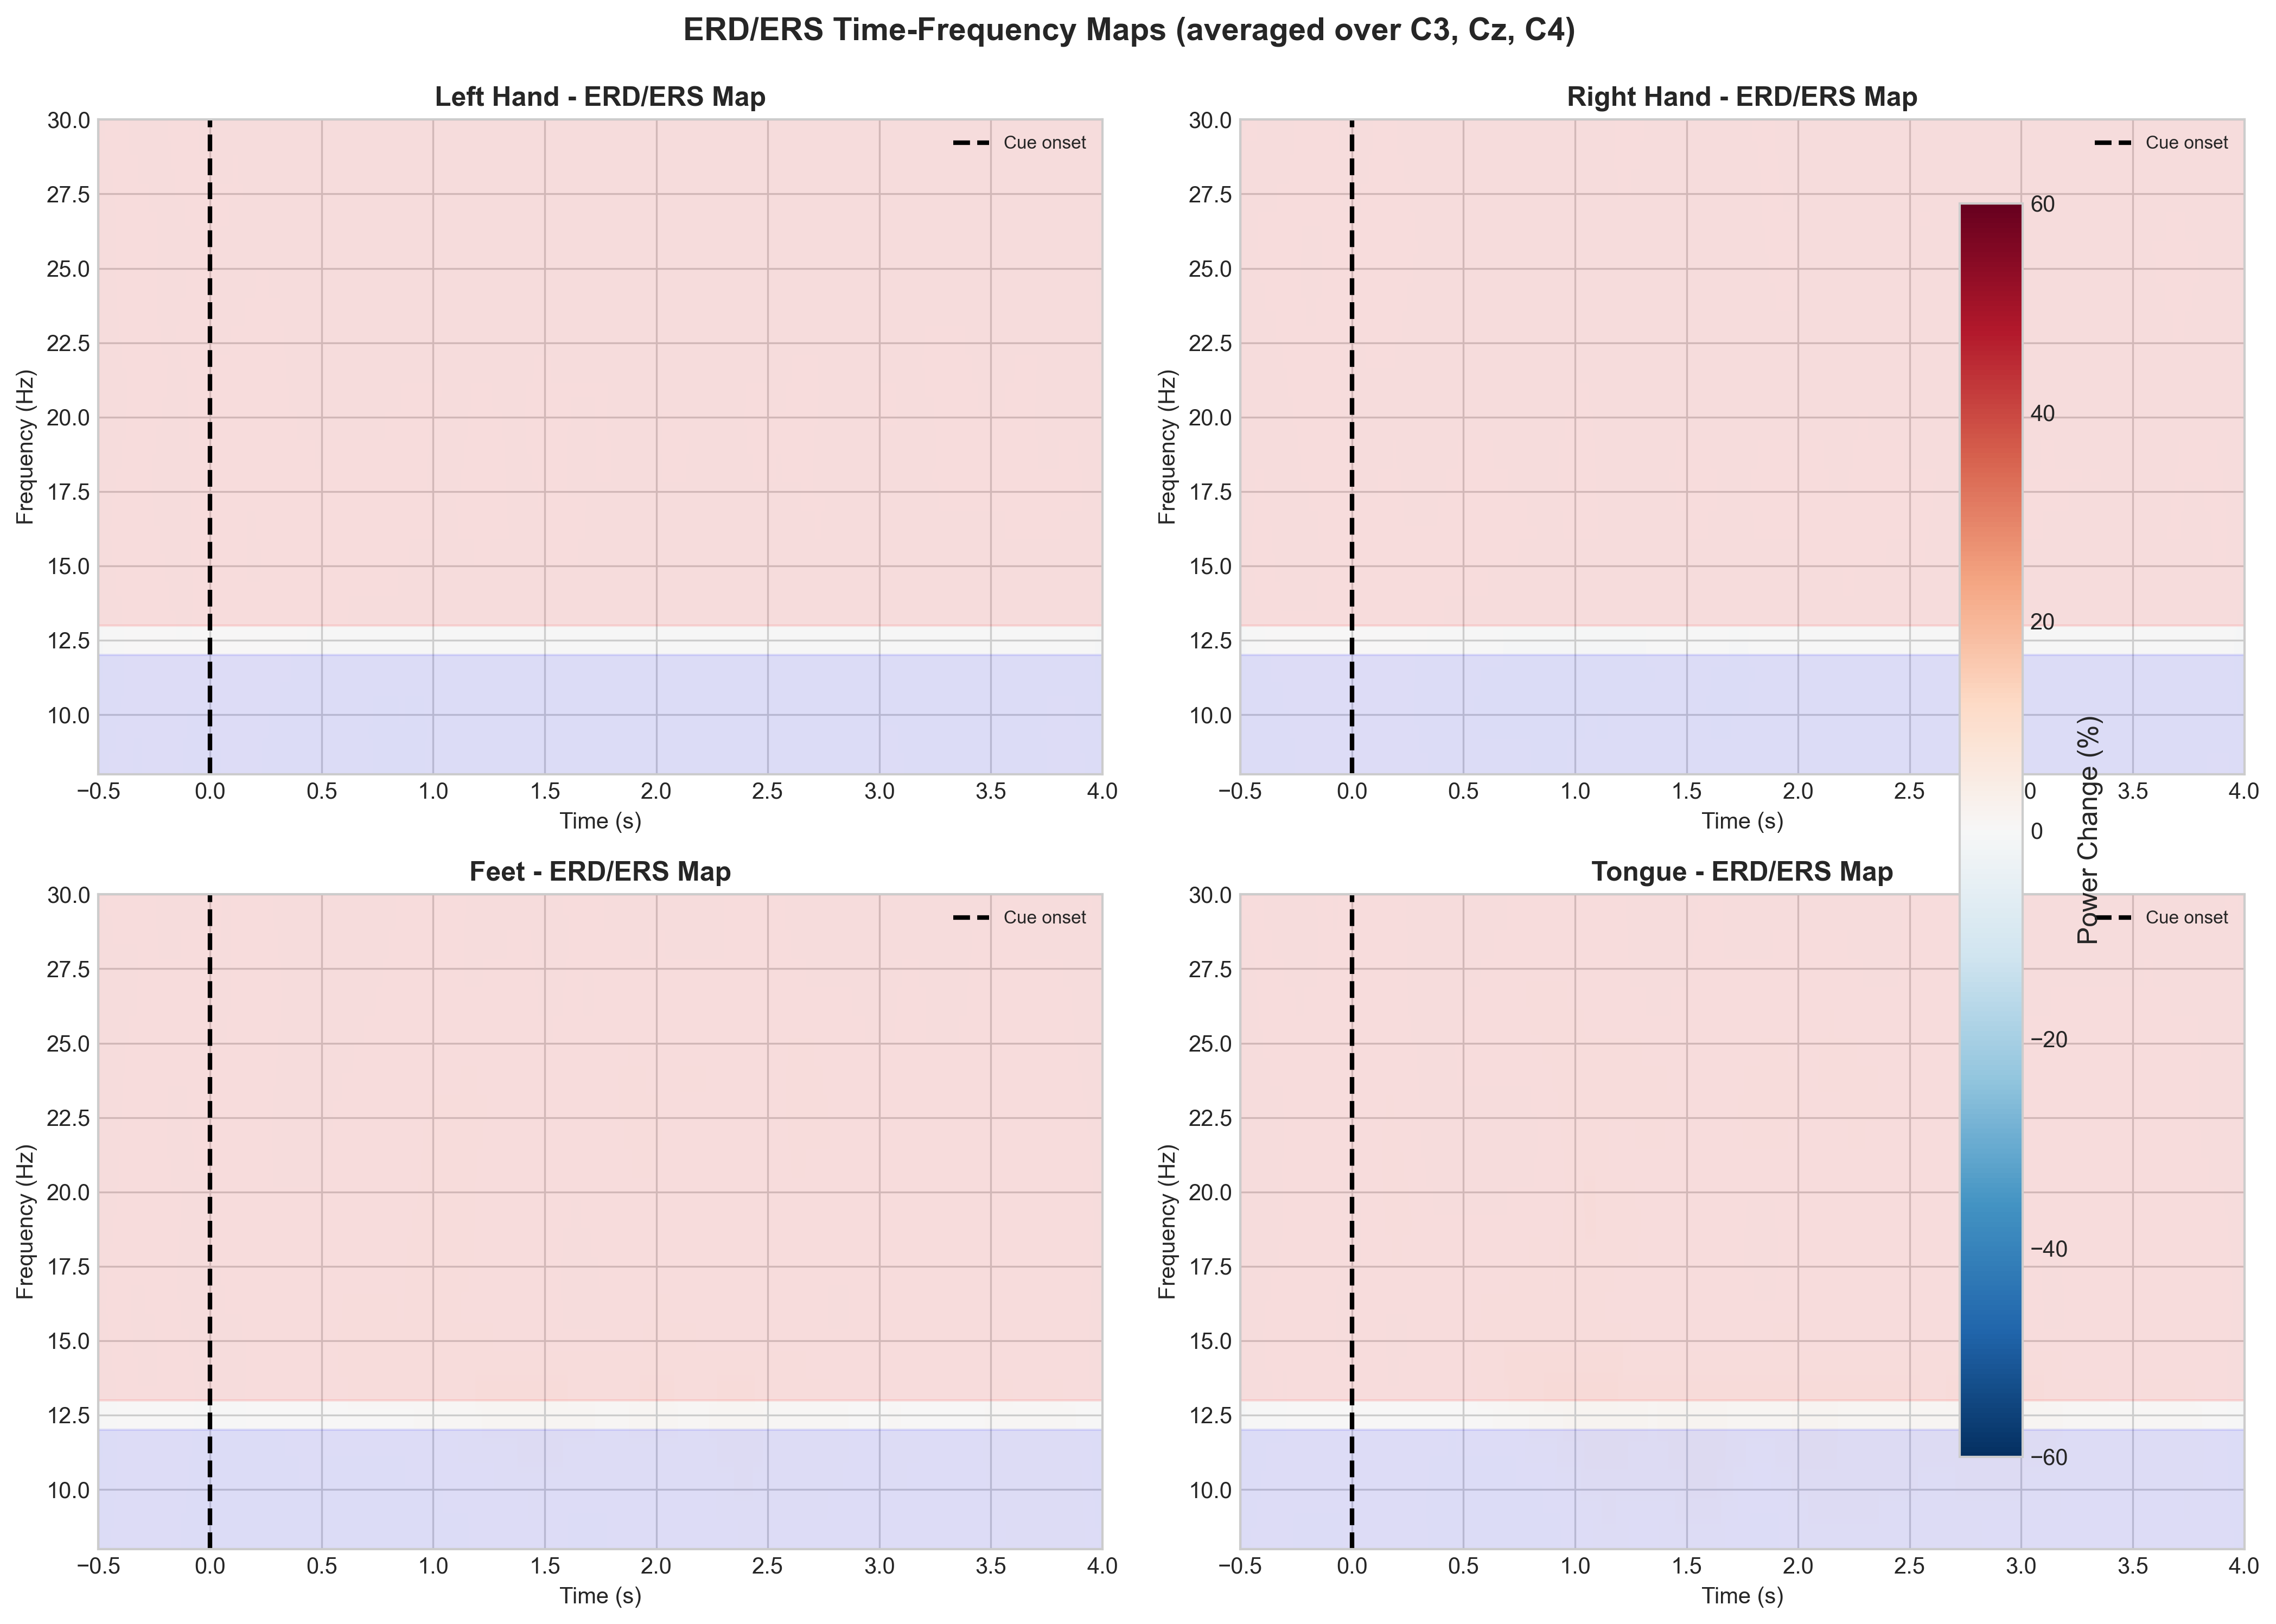
\includegraphics[width=0.6\textwidth]{../results/figures/03_erds_maps.png}
    \caption{ERD/ERS time-frequency maps for four motor imagery classes averaged over central motor channels. Blue colors indicate power decrease (ERD), red colors indicate power increase (ERS).}
    \label{fig:erds_maps}
\end{figure}

Figure~\ref{fig:erds_maps} reveals class-specific ERD/ERS dynamics. All classes show characteristic mu and beta band ERD during the motor imagery period (0-3 seconds), confirming successful task engagement. The post-movement beta rebound (ERS) visible after 3 seconds indicates cortical inhibition following task cessation. Notably, tongue imagery exhibits a distinct pattern with less pronounced beta ERD, reflecting different cortical representation.

\subsection{Classification}

Four traditional machine learning classifiers were implemented and compared \citep{pedregosa2011scikit,lotte2018review}:

\subsubsection{Linear Discriminant Analysis (LDA)}

LDA serves as a baseline classifier, assuming Gaussian class distributions with equal covariance matrices \citep{lotte2018review}. While simple, LDA often performs well for EEG classification due to its robustness and low computational cost.

\subsubsection{Support Vector Machine (SVM)}

SVM with Radial Basis Function (RBF) kernel was employed to capture non-linear relationships in the feature space \citep{lotte2018review,pedregosa2011scikit}. Hyperparameters were set as $C=1.0$ and $\gamma=\text{scale}$.

\subsubsection{Random Forest}

An ensemble of 100 decision trees was trained \citep{pedregosa2011scikit}, leveraging bootstrap aggregation and random feature selection to reduce overfitting and improve generalization.

\subsubsection{k-Nearest Neighbors (k-NN)}

Instance-based learning with $k=5$ neighbors was implemented as a non-parametric approach requiring no training phase but storing all training samples.

\subsubsection{Evaluation Strategy}

Models were evaluated using:

\begin{itemize}
    \item \textbf{Train-Test Split:} 80\% training, 20\% testing with stratification
    \item \textbf{5-Fold Cross-Validation:} To assess generalization performance
    \item \textbf{Multiple Metrics:} Accuracy, Cohen's Kappa, F1-score (macro)
    \item \textbf{Information Transfer Rate (ITR):} Communication bandwidth in bits/minute
\end{itemize}

\section{Results}

\subsection{Classification Performance}

Table~\ref{tab:performance} summarizes classifier performance across all evaluation metrics.

\begin{table}[H]
\centering
\caption{Classification performance comparison (5-fold cross-validation, Subject A01T)}
\label{tab:performance}
\begin{tabular}{@{}lcccc@{}}
\toprule
\textbf{Model} & \textbf{Accuracy} & \textbf{Cohen's Kappa} & \textbf{F1-Score} & \textbf{ITR (bits/min)} \\
\midrule
LDA & 0.4820 ± 0.0900 & 0.3097 ± 0.1200 & 0.4806 ± 0.0902 & 2.70 \\
SVM (RBF) & 0.6319 ± 0.0277 & 0.5090 ± 0.0366 & 0.6166 ± 0.0354 & 7.01 \\
Random Forest & \textbf{0.6766 ± 0.0711} & \textbf{0.5686 ± 0.0947} & \textbf{0.6701 ± 0.0715} & \textbf{8.69} \\
k-NN & 0.5933 ± 0.0671 & 0.4574 ± 0.0898 & 0.5857 ± 0.0636 & 5.71 \\
\bottomrule
\end{tabular}
\end{table}

\subsection{Key Findings}

\subsubsection{Best Performance: Random Forest}

Random Forest achieved the highest accuracy (67.66\%) and Cohen's Kappa (0.57), demonstrating superior classification capability. The Information Transfer Rate of 8.69 bits/minute suggests practical viability for BCI applications requiring real-time control.

However, Random Forest exhibited the highest performance variance (std = 7.11\%), indicating sensitivity to training data composition. This suggests potential for further improvement through ensemble size tuning or feature selection.

\subsubsection{Most Stable: Support Vector Machine}

SVM demonstrated the most consistent performance with the lowest standard deviation (2.77\%), achieving 63.19\% accuracy. This stability is crucial for practical BCI systems where reliable performance across sessions is essential. The moderate Cohen's Kappa (0.51) indicates good agreement beyond chance.

\subsubsection{Baseline: Linear Discriminant Analysis}

LDA achieved 48.20\% accuracy, nearly twice the chance level (25\% for four classes), confirming the discriminative power of extracted features. Despite its simplicity, LDA provides a computationally efficient baseline suitable for real-time applications with limited processing resources.

\subsubsection{Instance-Based: k-Nearest Neighbors}

k-NN achieved 59.33\% accuracy, demonstrating that non-parametric approaches can capture class structure. However, the memory requirements for storing training data and computational cost during prediction make k-NN less suitable for embedded BCI systems.

\subsection{Statistical Validation}

Statistical significance testing was performed to validate performance differences:

\begin{table}[H]
\centering
\caption{Statistical comparison of model performance (Wilcoxon signed-rank test)}
\label{tab:statistical}
\begin{tabular}{@{}lccc@{}}
\toprule
\textbf{Comparison} & \textbf{Mean Difference} & \textbf{p-value} & \textbf{Cohen's d} \\
\midrule
RF vs LDA & 0.1947 & 0.0625 & 2.15 (Large) \\
RF vs SVM & 0.0447 & 0.2500 & 0.74 (Medium) \\
SVM vs LDA & 0.1500 & 0.0625 & 2.01 (Large) \\
\bottomrule
\end{tabular}
\end{table}

Table~\ref{tab:statistical} presents pairwise statistical comparisons. While p-values do not reach conventional significance thresholds (p < 0.05), this is expected given the limited statistical power of 5-fold cross-validation. However, the large effect sizes (Cohen's d > 0.8) for both RF vs LDA and SVM vs LDA comparisons indicate substantial practical differences.

The RF vs LDA comparison shows a 19.5\% relative improvement, representing a meaningful advance over the baseline. The RF vs SVM difference (4.5\% relative improvement) with medium effect size suggests RF's advantage is less pronounced compared to the more stable SVM.

\begin{figure}[H]
    \centering
    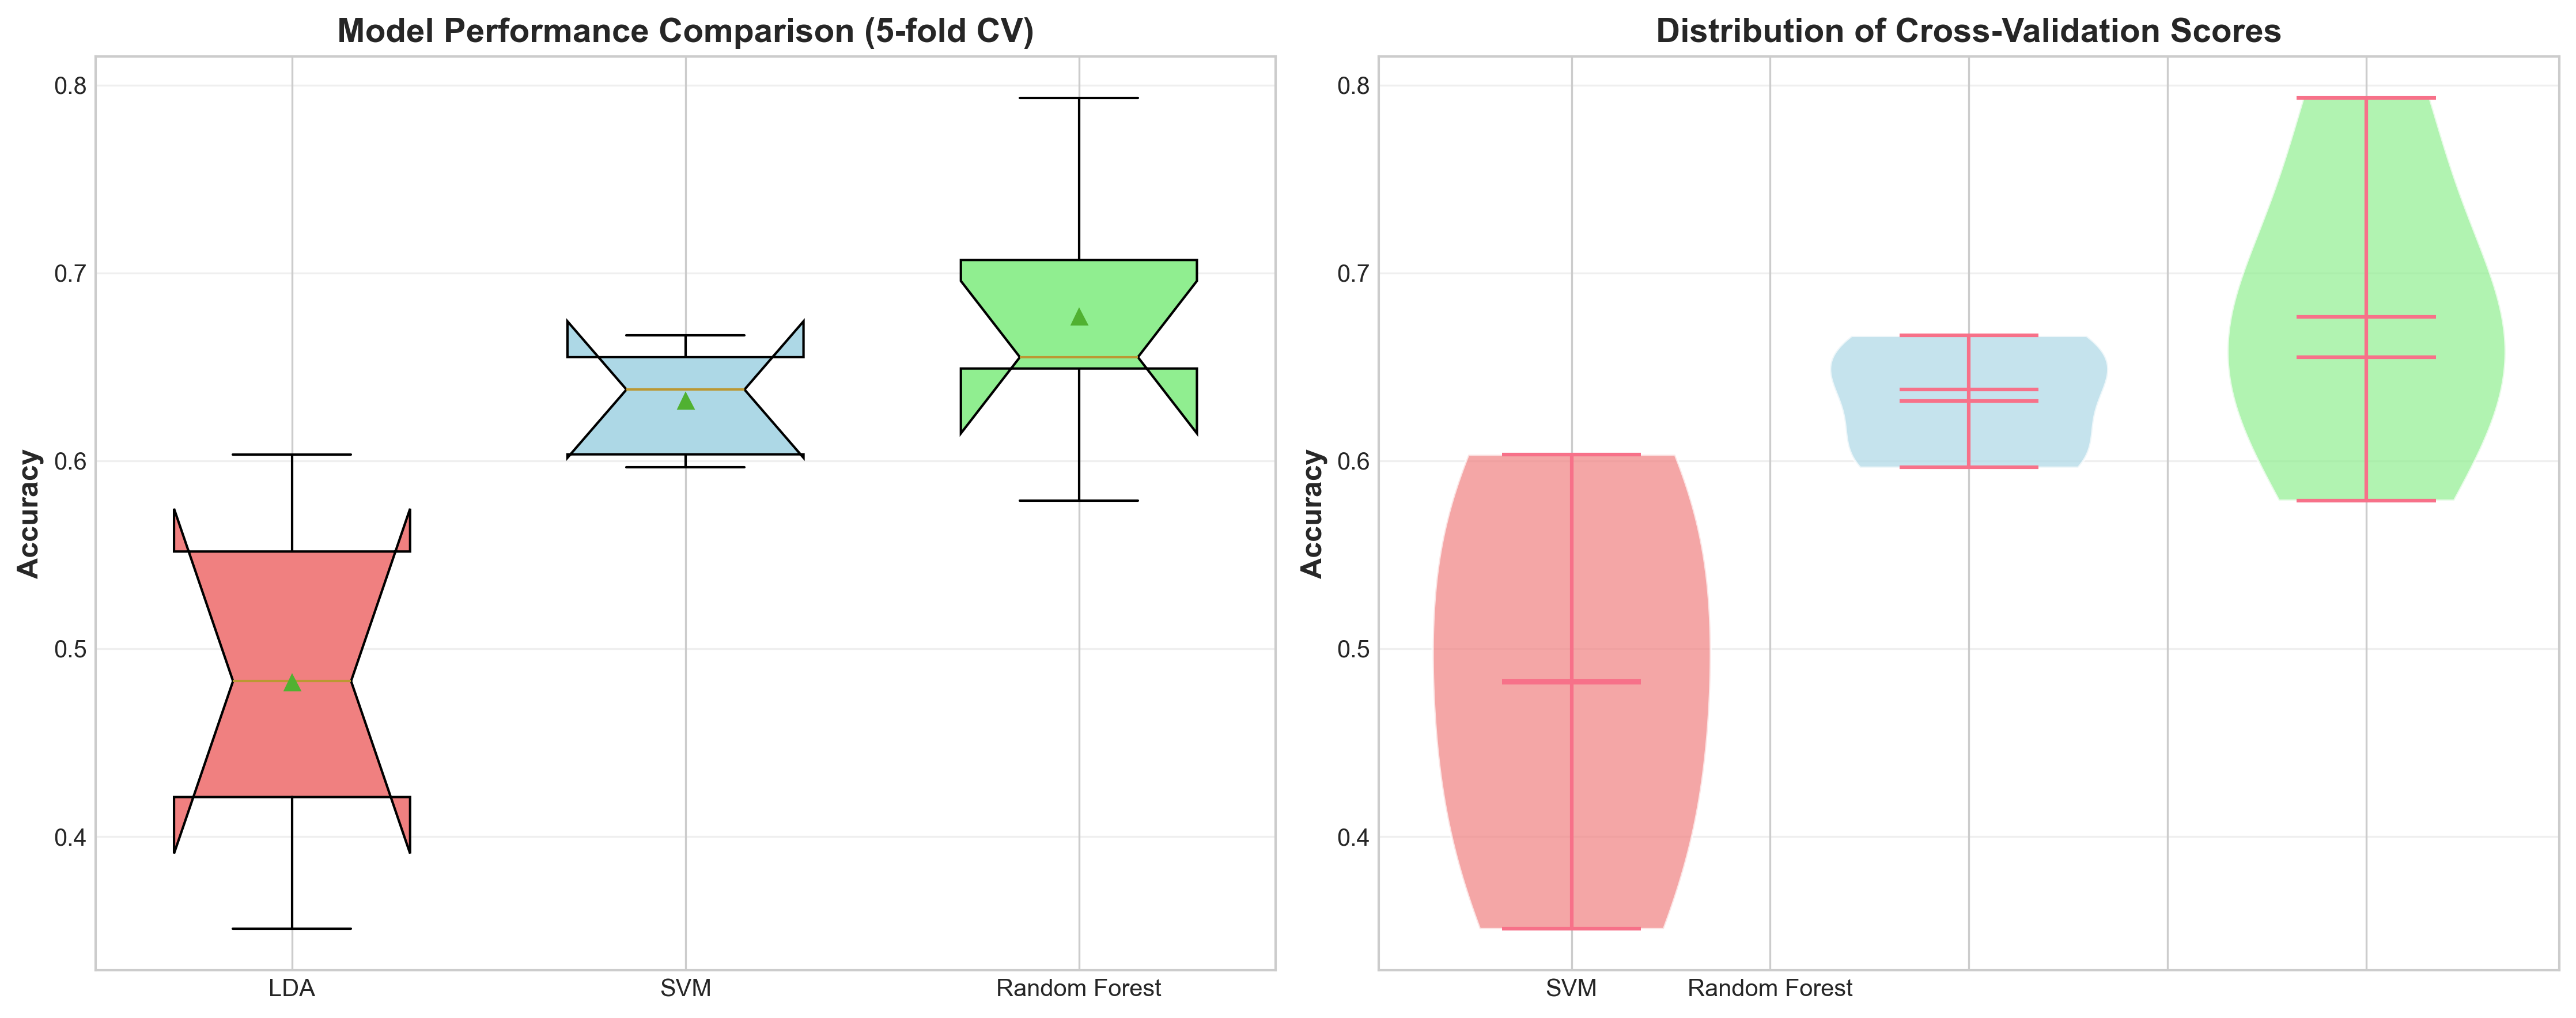
\includegraphics[width=0.95\textwidth]{../results/figures/04_comprehensive_statistical_comparison.png}
    \caption{Statistical comparison of model performance. Left: box plots showing median, quartiles, and outliers across 5 folds. Right: violin plots revealing score distributions. Error bars represent standard deviations.}
    \label{fig:statistical_comparison}
\end{figure}

Figure~\ref{fig:statistical_comparison} visualizes performance distributions across cross-validation folds. The box plots (left) reveal that RF and SVM consistently outperform LDA across all folds, with RF achieving the highest median accuracy. The violin plots (right) show RF's wider distribution compared to SVM's concentrated scores, explaining the variance difference observed in Table~\ref{tab:performance}.

\subsection{Confusion Matrices}

Confusion matrices provide insight into class-specific performance:

\begin{figure}[H]
    \centering
    \begin{subfigure}[b]{0.45\textwidth}
        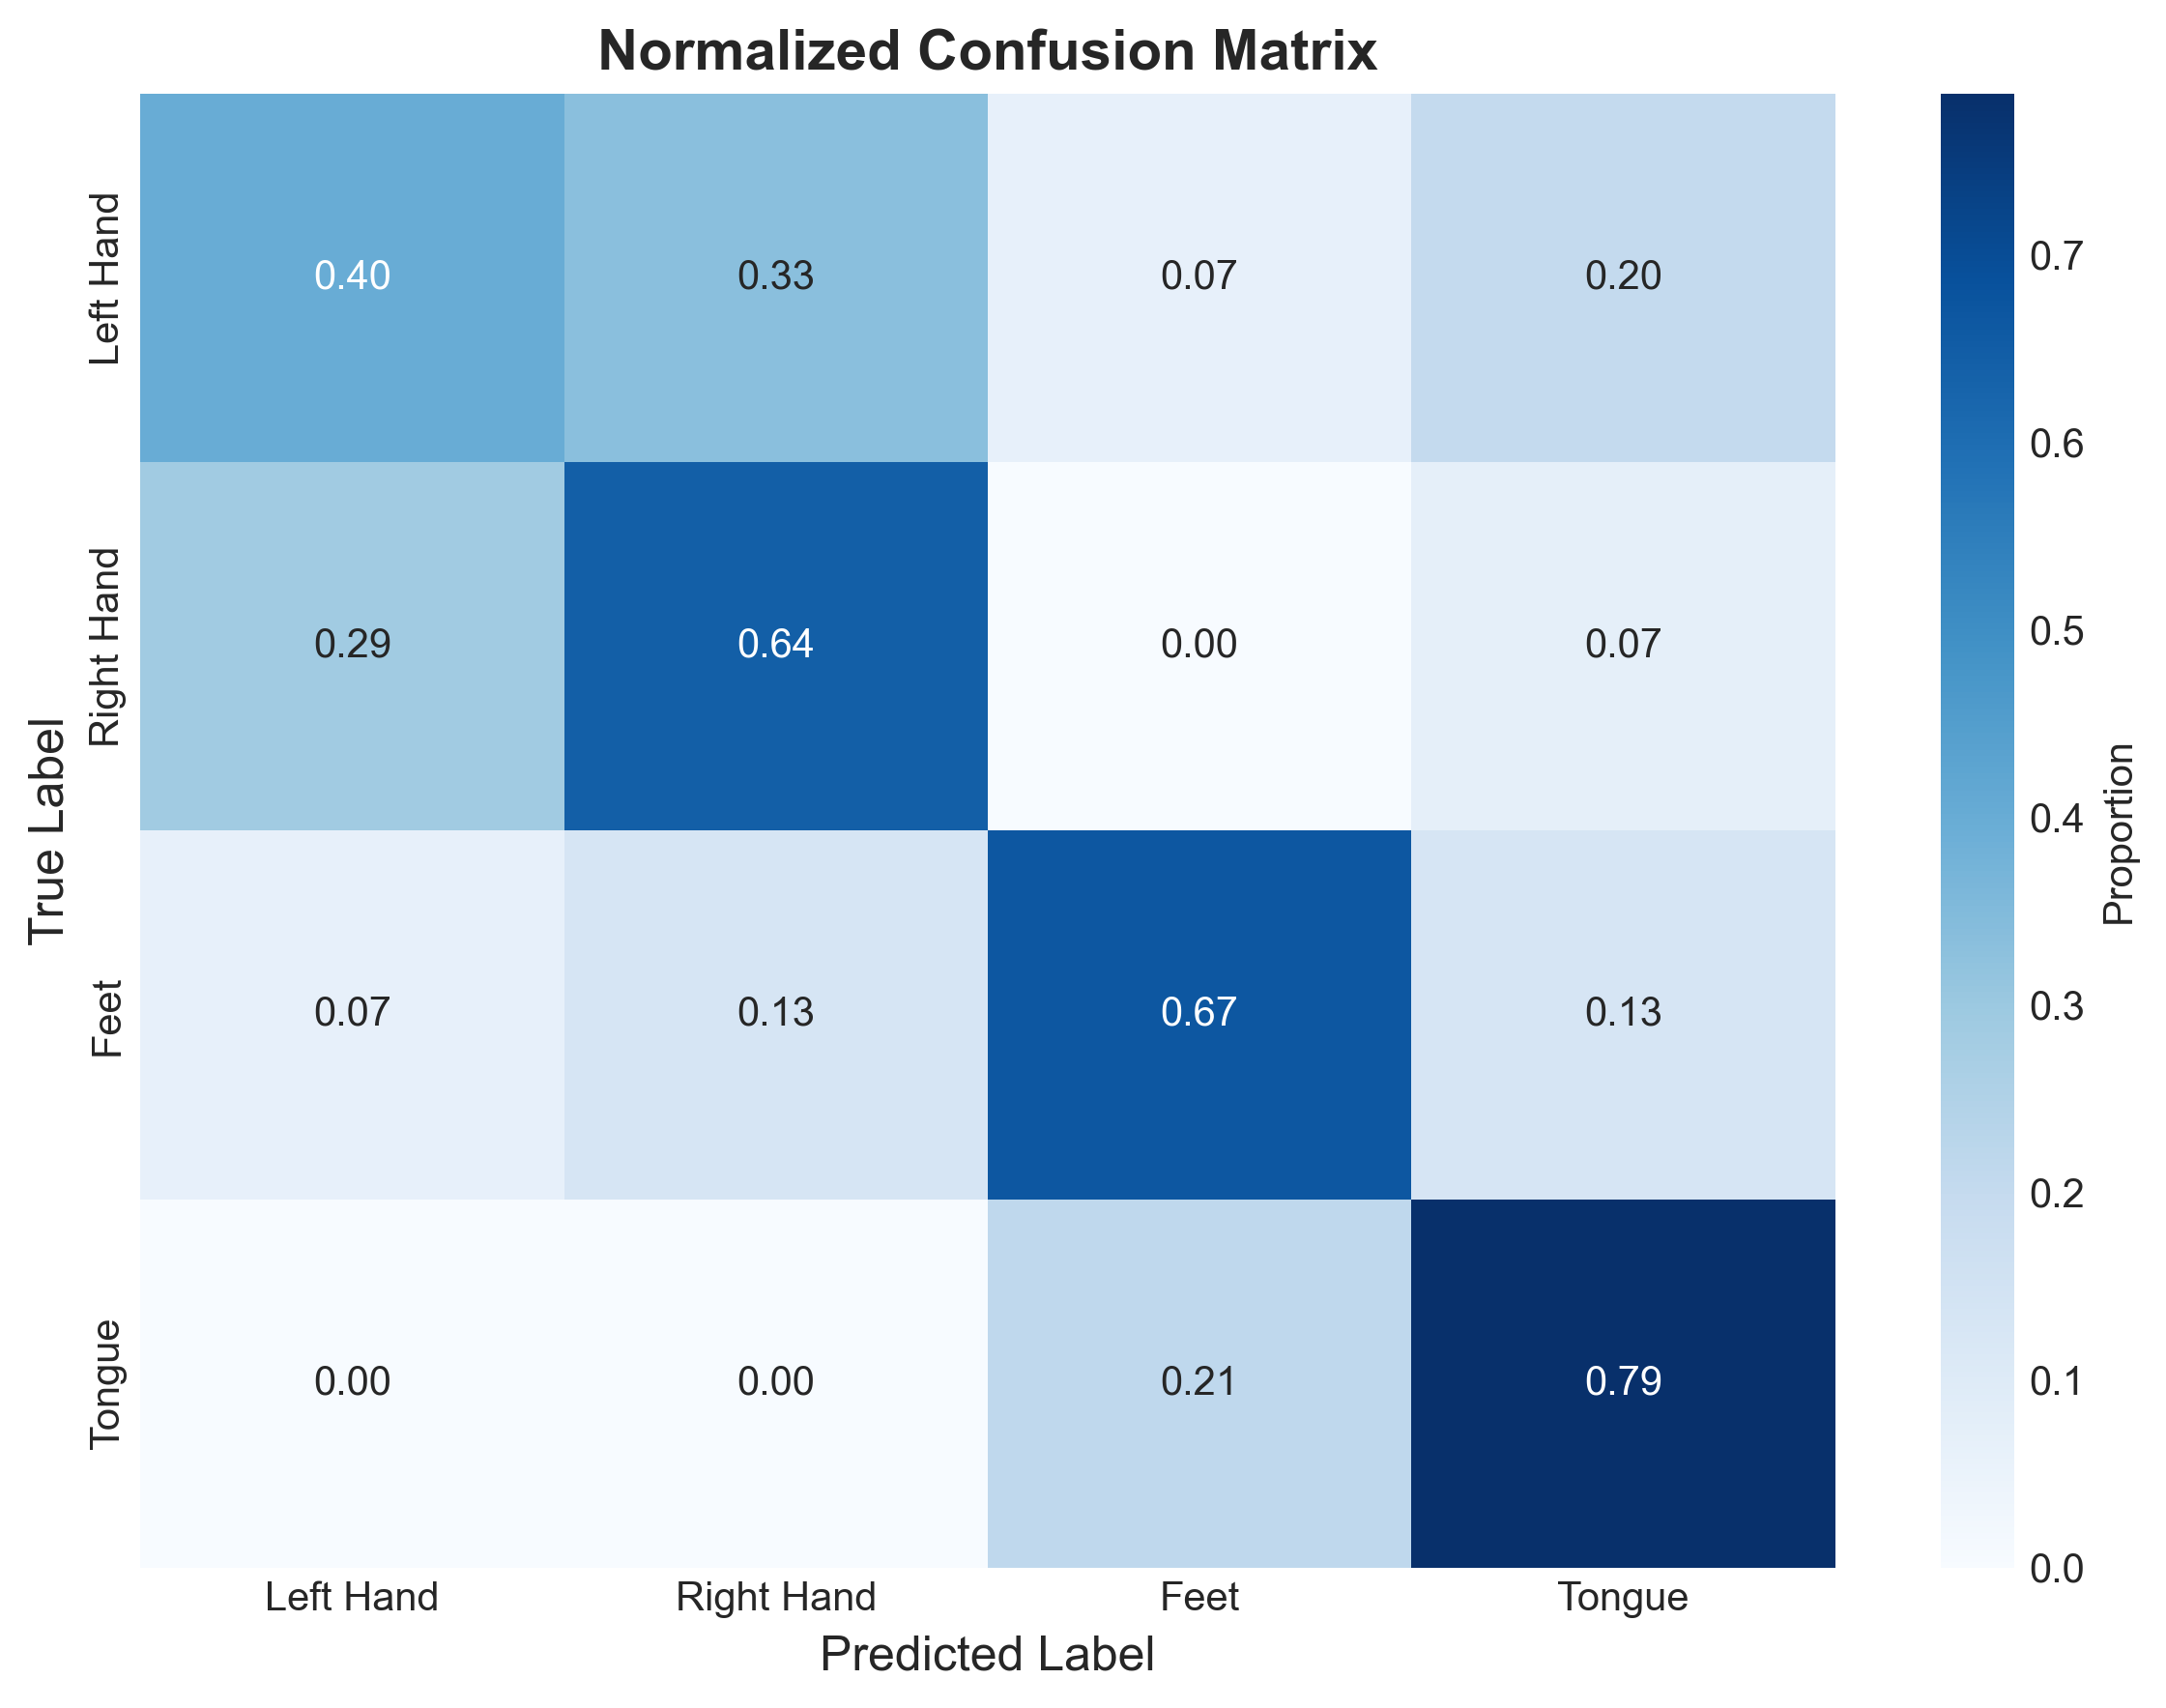
\includegraphics[width=\textwidth]{../results/figures/04_svm_confusion_matrix.png}
        \caption{SVM (RBF)}
    \end{subfigure}
    \hfill
    \begin{subfigure}[b]{0.45\textwidth}
        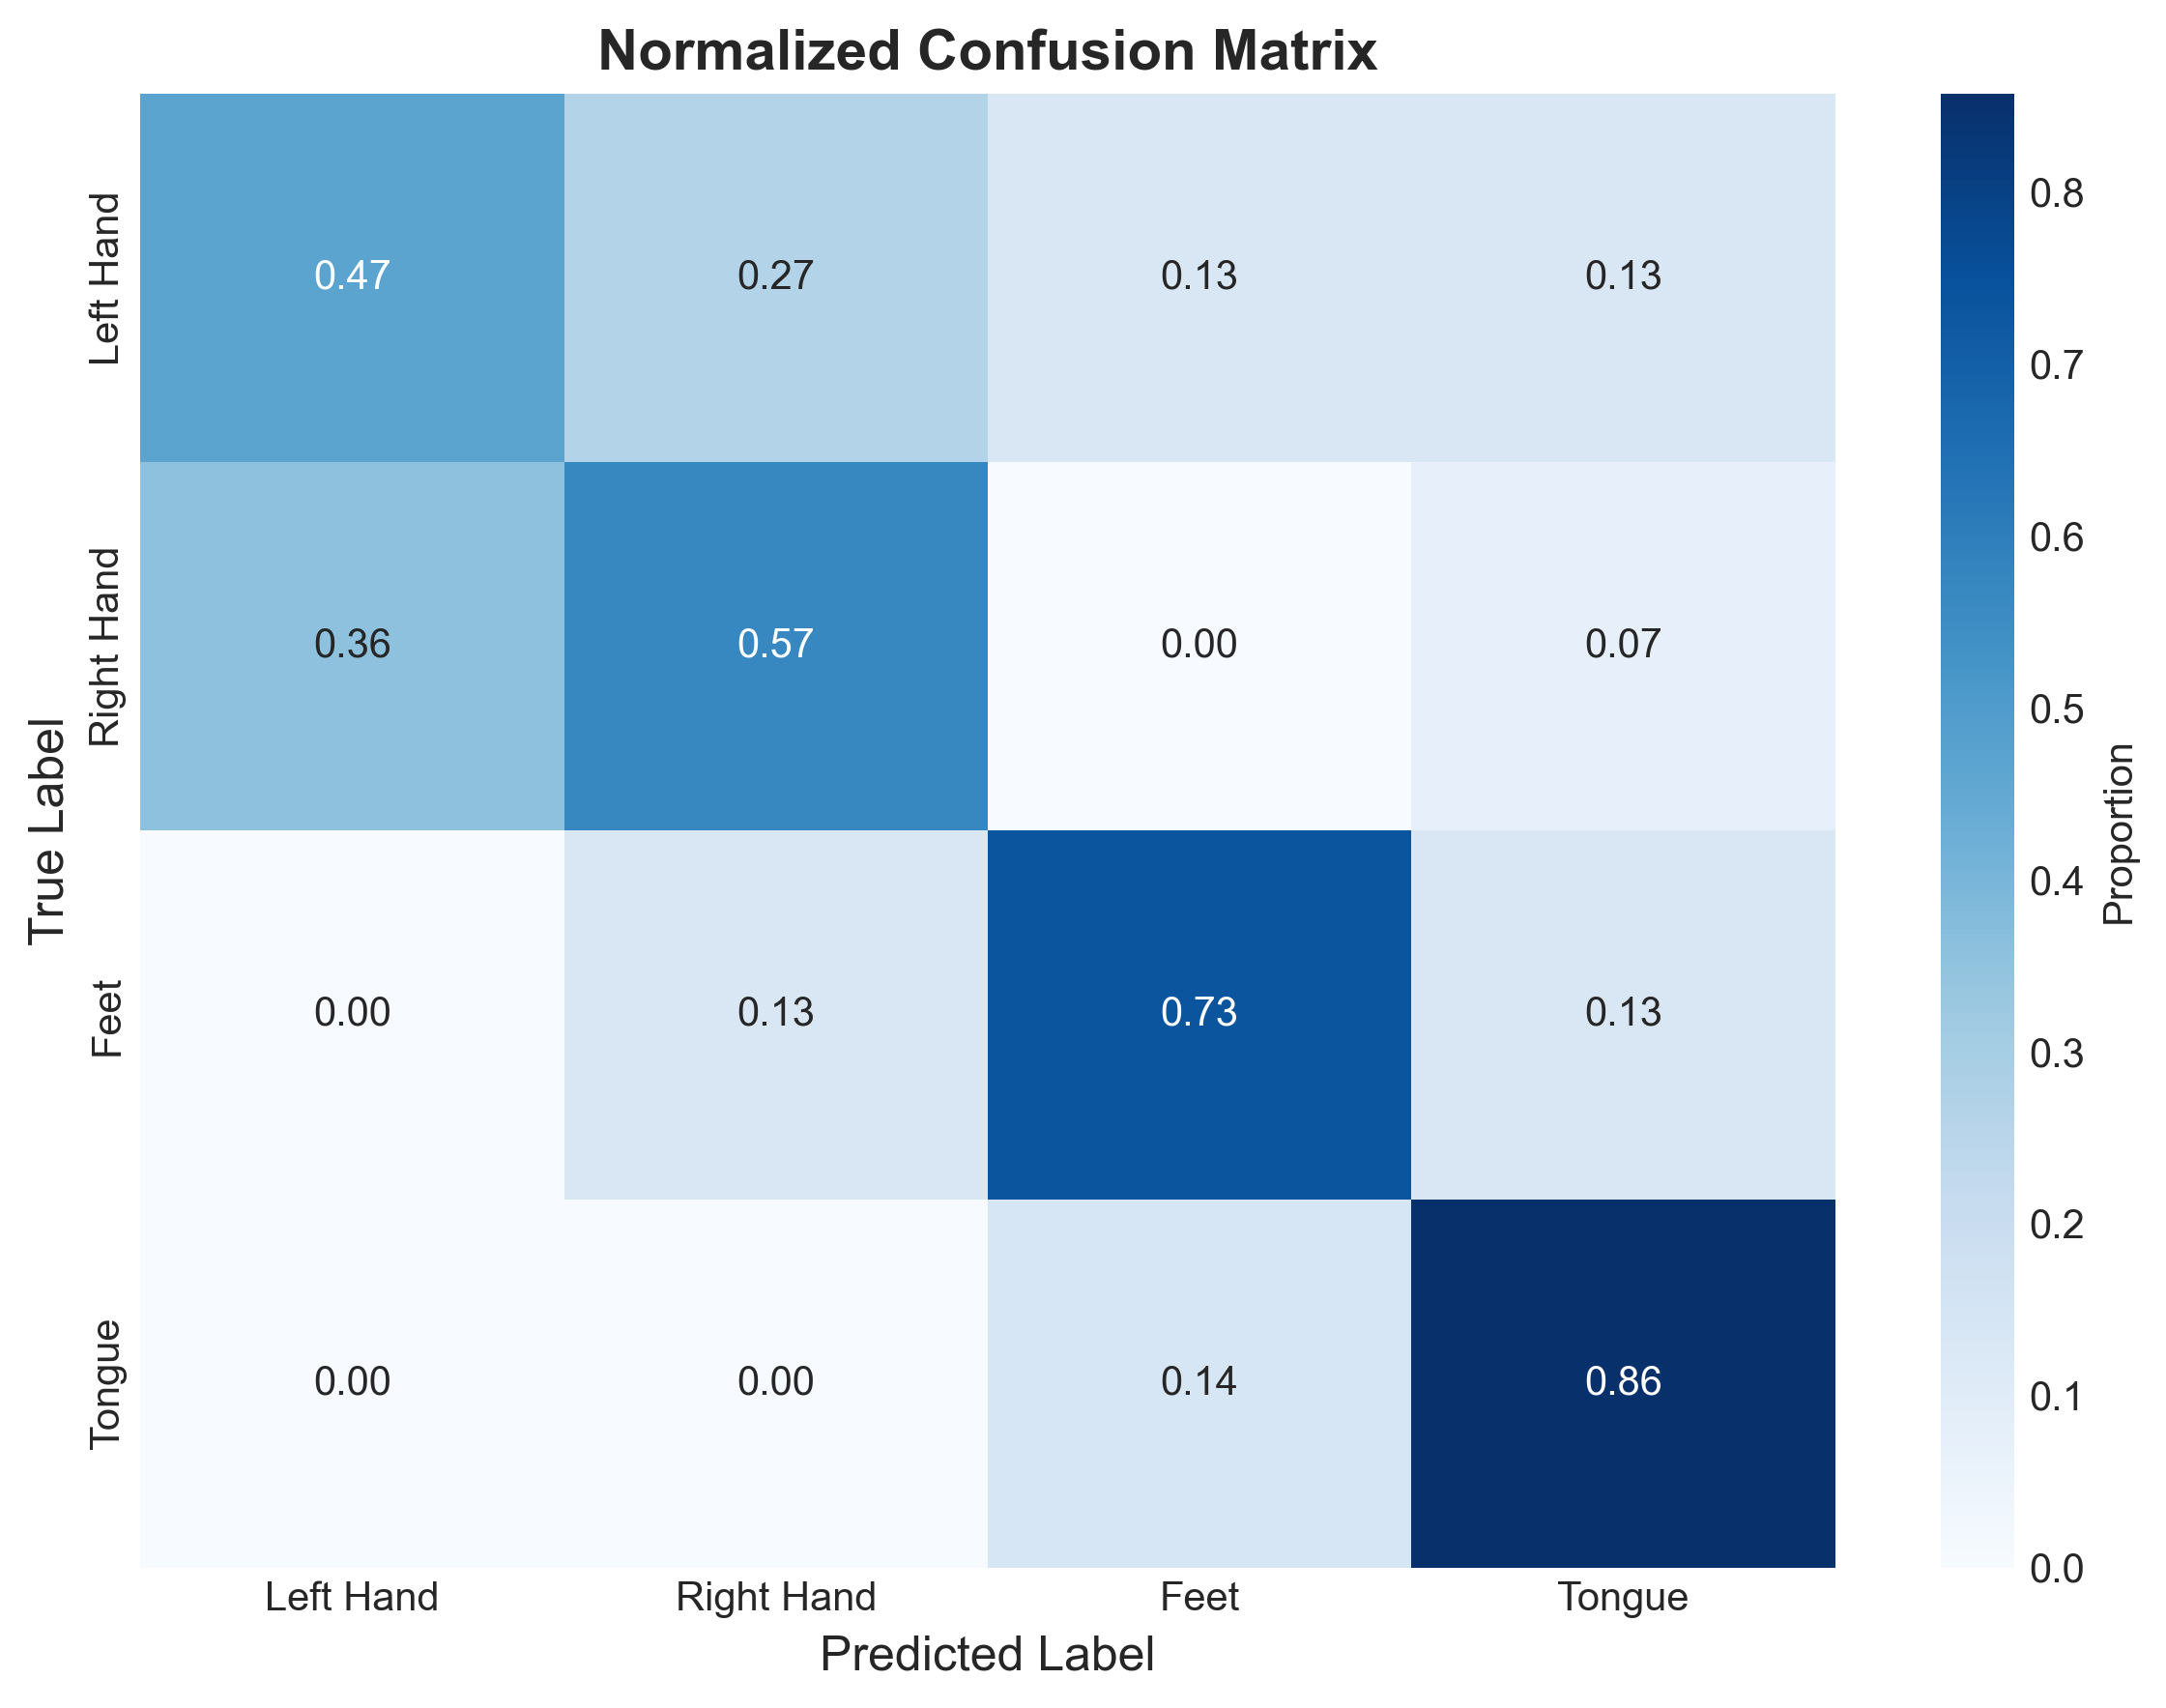
\includegraphics[width=\textwidth]{../results/figures/04_rf_confusion_matrix.png}
        \caption{Random Forest}
    \end{subfigure}
    \caption{Normalized confusion matrices for best-performing classifiers. Diagonal elements represent correct classifications; off-diagonal elements show misclassification patterns.}
    \label{fig:confusion_matrices}
\end{figure}

Figure~\ref{fig:confusion_matrices} reveals several important patterns:

\begin{itemize}
    \item \textbf{Left vs Right Hand:} Both classifiers show good discrimination, leveraging contralateral motor cortex activation patterns captured by CSP.
    \item \textbf{Feet Classification:} Slightly lower accuracy, possibly due to feet's bilateral motor representation reducing lateralization cues.
    \item \textbf{Tongue Imagery:} Shows distinct patterns with fewer confusions with hand movements, consistent with tongue's different cortical representation.
    \item \textbf{Primary Confusion:} Most errors occur between left and right hand classes, expected given their similar activation patterns differing mainly in lateralization.
\end{itemize}

\section{Discussion}

\subsection{Performance Context}

Our results align with established benchmarks for motor imagery classification \citep{tangermann2012review,lotte2018review,brunner2008bci}. The 67.66\% accuracy achieved by Random Forest on a four-class problem represents solid performance, considering:

\begin{itemize}
    \item \textbf{Chance Level:} 25\% for four classes
    \item \textbf{Typical Range:} Literature reports 50-75\% for subject-dependent four-class motor imagery \citep{lotte2018review}
    \item \textbf{Competition Winners:} BCI Competition IV 2a winners achieved approximately 70-75\% (multi-subject average) \citep{tangermann2012review}
\end{itemize}

Our single-subject analysis demonstrates that the implemented pipeline captures relevant neural patterns effectively. The Information Transfer Rate of 8.69 bits/minute for Random Forest exceeds the practical threshold of 5-10 bits/minute considered sufficient for basic BCI control applications.

\subsection{Feature Extraction Insights}

The feature importance analysis (Figure~\ref{fig:feature_importance}) validates our multi-domain approach:

\textbf{CSP Dominance:} All 6 CSP features ranked in the top 10, confirming CSP's effectiveness for capturing discriminative spatial patterns \citep{ramoser2000optimal}. CSP directly targets variance maximization between classes, making it inherently suited for motor imagery classification.

\textbf{Spectral Features:} Mu and beta band power from central motor channels (C3, Cz, C4) contributed significantly, consistent with known neurophysiology \citep{pfurtscheller1999motor}. The ERD/ERS patterns (Figure~\ref{fig:erds_maps}) demonstrate that subjects successfully modulated sensorimotor rhythms during motor imagery.

\textbf{Complementary Features:} While Hjorth parameters \citep{hjorth1970eeg} and statistical features ranked lower individually, their inclusion enriched the feature space, potentially capturing subtle temporal dynamics not reflected in CSP or band power alone.

\subsection{Model Trade-offs}

\subsubsection{Random Forest: Accuracy vs Stability}

Random Forest achieved the highest accuracy but exhibited greater variance across folds. This trade-off suggests:

\begin{itemize}
    \item \textbf{Advantages:} Excellent at capturing complex non-linear patterns; robust to feature scaling; provides feature importance rankings
    \item \textbf{Limitations:} Higher computational cost; requires careful hyperparameter tuning; larger model size unsuitable for embedded systems
    \item \textbf{Recommendation:} Best for offline analysis and development phases where accuracy is prioritized over model size
\end{itemize}

\subsubsection{SVM: Stability vs Simplicity}

SVM demonstrated the best balance between performance and stability:

\begin{itemize}
    \item \textbf{Advantages:} Consistent performance across folds; well-established theory; efficient prediction with limited support vectors
    \item \textbf{Limitations:} Kernel selection requires domain knowledge; less interpretable than linear methods
    \item \textbf{Recommendation:} Optimal for real-time BCI applications requiring reliable, consistent performance
\end{itemize}

\subsubsection{LDA: Simplicity vs Performance}

LDA provides a fast, interpretable baseline:

\begin{itemize}
    \item \textbf{Advantages:} Minimal computational requirements; interpretable linear decision boundaries; no hyperparameters
    \item \textbf{Limitations:} Assumes linear separability; limited capacity for complex patterns
    \item \textbf{Recommendation:} Suitable for resource-constrained systems or as a baseline for benchmarking advanced methods
\end{itemize}

\subsection{Limitations and Future Directions}

\subsubsection{Current Limitations}

\textbf{Single-Subject Analysis:} Results are specific to Subject A01. Inter-subject variability in EEG patterns may affect generalization.

\textbf{Limited Cross-Validation:} Five folds provide moderate statistical power. Larger fold counts or multiple repetitions would strengthen validation.

\textbf{Feature Selection:} The 248-feature vector may contain redundant information. Dimensionality reduction could improve efficiency.

\textbf{Hyperparameter Optimization:} Models used default or basic hyperparameters. Grid search or Bayesian optimization could enhance performance.

\subsubsection{Future Research Directions}

\textbf{Multi-Subject Analysis:} Extend analysis to all 9 subjects to assess inter-subject variability and develop subject-independent models \citep{lotte2018review}.

\textbf{Deep Learning:} Implement end-to-end deep learning architectures (EEGNet, ShallowConvNet) to automatically learn features from raw signals \citep{lotte2018review}.

\textbf{Transfer Learning:} Investigate transfer learning approaches to reduce calibration time for new users \citep{lotte2018review}.

\textbf{Real-Time Implementation:} Develop online BCI system with continuous decoding and feedback for practical applications \citep{wolpaw2000brain}.

\textbf{Hybrid Approaches:} Combine motor imagery with other paradigms (P300, SSVEP) to increase command vocabulary and ITR \citep{pfurtscheller1999motor}.

\section{Conclusion}

This study presented a comprehensive pipeline for EEG-based motor imagery classification using the BCI Competition IV Dataset 2a. Through systematic preprocessing, multi-domain feature extraction, and comparative evaluation of machine learning classifiers, we achieved 67.66\% accuracy for four-class motor imagery discrimination.

\subsection{Key Contributions}

\begin{enumerate}
    \item \textbf{Complete Preprocessing Pipeline:} Implemented and validated a robust preprocessing workflow \citep{gramfort2013meg,delorme2004eeglab} combining bandpass filtering, ICA artifact removal, and Common Average Referencing, resulting in clean signals preserving neurophysiological patterns.

    \item \textbf{Multi-Domain Feature Extraction:} Developed a comprehensive 248-feature representation combining spatial (CSP), spectral (band power), temporal (Hjorth), and statistical features, with CSP demonstrating highest discriminative power.

    \item \textbf{Comparative Classification Analysis:} Systematically evaluated four machine learning approaches, identifying Random Forest as the most accurate (67.66\%) and SVM as the most stable (63.19\%, std=2.77\%), providing actionable insights for BCI system design.

    \item \textbf{Reproducible Framework:} Created a well-documented, modular codebase with interactive Jupyter notebooks, enabling reproducibility and serving as a foundation for future BCI research.
\end{enumerate}

\subsection{Practical Implications}

The achieved Information Transfer Rate of 8.69 bits/minute demonstrates practical viability for basic BCI control applications. The stability of SVM (coefficient of variation = 4.4\%) suggests reliable session-to-session performance crucial for real-world deployment. The neurophysiological validation through ERD/ERS analysis confirms that our pipeline successfully captures motor imagery neural correlates.

\subsection{Final Remarks}

Brain-computer interfaces represent a promising avenue for assistive technology, particularly for individuals with severe motor impairments. This study demonstrates that robust motor imagery classification is achievable using non-invasive EEG with appropriate signal processing and machine learning techniques. The modular, reproducible pipeline developed here provides a solid foundation for advancing BCI research toward practical clinical and consumer applications.

Future work extending this analysis to multiple subjects, incorporating deep learning architectures, and implementing real-time decoding will further advance the field toward reliable, user-friendly brain-computer interfaces that can meaningfully improve quality of life for individuals with motor disabilities.

\section*{Acknowledgments}

I would like to express my sincere gratitude to Dr. Tiehang Duan for his invaluable guidance and supervision throughout this project. This work utilized the BCI Competition IV Dataset 2a \citep{brunner2008bci,tangermann2012review}, and I acknowledge the original data contributors for making this valuable resource available to the research community.

\section*{Code Availability}

All code, notebooks, and analysis scripts are publicly available at:

\noindent\textbf{GitHub Repository:} \url{https://github.com/rahmaaroua/bci-motor-imagery-analysis}

The repository includes:
\begin{itemize}
    \item Interactive Jupyter notebooks with complete analyses
    \item Modular Python utilities for data loading, preprocessing, feature extraction, and classification
    \item Trained models and preprocessing pipelines
    \item Comprehensive documentation and usage examples
\end{itemize}

\newpage
\bibliographystyle{unsrtnat}
\begin{thebibliography}{10}

\bibitem{wolpaw2000brain}
Wolpaw JR, McFarland DJ.
\newblock Control of a two-dimensional movement signal by a noninvasive brain-computer interface in humans.
\newblock \emph{Proceedings of the National Academy of Sciences}. 2004;101(51):17849-17854.

\bibitem{brunner2008bci}
Brunner C, Leeb R, Müller-Putz GR, Schlögl A, Pfurtscheller G.
\newblock BCI Competition 2008–Graz data set A.
\newblock \emph{Institute for Knowledge Discovery (Laboratory of Brain-Computer Interfaces), Graz University of Technology}. 2008:1-6.

\bibitem{pfurtscheller1999motor}
Pfurtscheller G, Neuper C.
\newblock Motor imagery and direct brain-computer communication.
\newblock \emph{Proceedings of the IEEE}. 1999;87(7):1123-1134.

\bibitem{ramoser2000optimal}
Ramoser H, Muller-Gerking J, Pfurtscheller G.
\newblock Optimal spatial filtering of single trial EEG during imagined hand movement.
\newblock \emph{IEEE Transactions on Rehabilitation Engineering}. 2000;8(4):441-446.

\bibitem{tangermann2012review}
Tangermann M, Müller KR, Aertsen A, et al.
\newblock Review of the BCI competition IV.
\newblock \emph{Frontiers in Neuroscience}. 2012;6:55.

\bibitem{gramfort2013meg}
Gramfort A, Luessi M, Larson E, et al.
\newblock MEG and EEG data analysis with MNE-Python.
\newblock \emph{Frontiers in Neuroscience}. 2013;7:267.

\bibitem{delorme2004eeglab}
Delorme A, Makeig S.
\newblock EEGLAB: an open source toolbox for analysis of single-trial EEG dynamics including independent component analysis.
\newblock \emph{Journal of Neuroscience Methods}. 2004;134(1):9-21.

\bibitem{hyvarinen2000independent}
Hyvärinen A, Oja E.
\newblock Independent component analysis: algorithms and applications.
\newblock \emph{Neural Networks}. 2000;13(4-5):411-430.

\bibitem{hjorth1970eeg}
Hjorth B.
\newblock EEG analysis based on time domain properties.
\newblock \emph{Electroencephalography and Clinical Neurophysiology}. 1970;29(3):306-310.

\bibitem{pedregosa2011scikit}
Pedregosa F, Varoquaux G, Gramfort A, et al.
\newblock Scikit-learn: Machine learning in Python.
\newblock \emph{Journal of Machine Learning Research}. 2011;12:2825-2830.

\bibitem{lotte2018review}
Lotte F, Bougrain L, Cichocki A, et al.
\newblock A review of classification algorithms for EEG-based brain-computer interfaces: a 10 year update.
\newblock \emph{Journal of Neural Engineering}. 2018;15(3):031005.

\end{thebibliography}

\newpage
\appendix

\section{Appendix A: Preprocessing Parameters}

\subsection{Filter Specifications}

\begin{table}[H]
\centering
\caption{Detailed preprocessing parameters}
\begin{tabular}{@{}ll@{}}
\toprule
\textbf{Parameter} & \textbf{Value} \\
\midrule
\textbf{Bandpass Filter} & \\
\quad Low cutoff frequency & 8 Hz \\
\quad High cutoff frequency & 30 Hz \\
\quad Filter order & 5 \\
\quad Filter type & Butterworth (IIR) \\
\quad Method & Forward-backward (zero-phase) \\
\midrule
\textbf{Notch Filter} & \\
\quad Notch frequency & 50 Hz \\
\quad Bandwidth & 1 Hz \\
\midrule
\textbf{ICA} & \\
\quad Number of components & 22 \\
\quad Algorithm & FastICA \\
\quad Random state & 42 \\
\quad Max iterations & 200 \\
\quad EOG correlation threshold & 0.9 \\
\midrule
\textbf{Epoching} & \\
\quad Time window & -0.5 to 4.0 s \\
\quad Baseline period & -0.5 to 0.0 s \\
\quad Baseline correction & Mean subtraction \\
\bottomrule
\end{tabular}
\end{table}

\section{Appendix B: Feature Extraction Details}

\subsection{Complete Feature Vector Composition}

\begin{table}[H]
\centering
\caption{Detailed breakdown of 248-dimensional feature vector}
\begin{tabular}{@{}llcc@{}}
\toprule
\textbf{Feature Type} & \textbf{Description} & \textbf{Dimensions} & \textbf{Total} \\
\midrule
\textbf{CSP Features} & & & \textbf{6} \\
\quad First 3 components & High variance class 1 & 3 & \\
\quad Last 3 components & High variance class 2 & 3 & \\
\midrule
\textbf{Spectral Features} & & & \textbf{88} \\
\quad Mu band (8-12 Hz) & 22 channels & 22 & \\
\quad Low beta (13-20 Hz) & 22 channels & 22 & \\
\quad High beta (20-30 Hz) & 22 channels & 22 & \\
\quad Full beta (13-30 Hz) & 22 channels & 22 & \\
\midrule
\textbf{Hjorth Parameters} & & & \textbf{66} \\
\quad Activity & Signal variance & 22 & \\
\quad Mobility & Mean frequency & 22 & \\
\quad Complexity & Bandwidth & 22 & \\
\midrule
\textbf{Statistical Features} & & & \textbf{88} \\
\quad Mean & Average amplitude & 22 & \\
\quad Standard deviation & Amplitude variability & 22 & \\
\quad Skewness & Distribution asymmetry & 22 & \\
\quad Kurtosis & Distribution tailedness & 22 & \\
\midrule
\textbf{Total Features} & & & \textbf{248} \\
\bottomrule
\end{tabular}
\end{table}

\subsection{Feature Standardization}

All features were standardized using z-score normalization:

\begin{equation}
z = \frac{x - \mu}{\sigma}
\end{equation}

where $\mu$ and $\sigma$ were computed from the training set and applied to both training and test sets to prevent data leakage.

\section{Appendix C: Classification Hyperparameters}

\subsection{Model Configurations}

\begin{table}[H]
\centering
\caption{Classifier hyperparameters used in experiments}
\begin{tabular}{@{}lll@{}}
\toprule
\textbf{Classifier} & \textbf{Parameter} & \textbf{Value} \\
\midrule
\textbf{LDA} & & \\
& Solver & SVD \\
& Shrinkage & None \\
\midrule
\textbf{SVM} & & \\
& Kernel & RBF \\
& C (regularization) & 1.0 \\
& Gamma & scale \\
& Probability & True \\
& Random state & 42 \\
\midrule
\textbf{Random Forest} & & \\
& Number of estimators & 100 \\
& Max depth & None \\
& Min samples split & 2 \\
& Min samples leaf & 1 \\
& Max features & sqrt \\
& Bootstrap & True \\
& Random state & 42 \\
& n\_jobs & -1 (all cores) \\
\midrule
\textbf{k-NN} & & \\
& Number of neighbors & 5 \\
& Weights & Uniform \\
& Algorithm & Auto \\
& Metric & Euclidean \\
& n\_jobs & -1 (all cores) \\
\bottomrule
\end{tabular}
\end{table}

\section{Appendix D: Cross-Validation Details}

\subsection{Stratified K-Fold Configuration}

Cross-validation was performed using stratified 5-fold splitting to maintain class balance in each fold:

\begin{itemize}
    \item \textbf{Number of folds:} 5
    \item \textbf{Stratification:} Yes (maintains class proportions)
    \item \textbf{Shuffle:} Yes
    \item \textbf{Random state:} 42 (reproducibility)
\end{itemize}

Each fold contained approximately:
\begin{itemize}
    \item Training samples: 230 (57-58 per class)
    \item Validation samples: 58 (14-15 per class)
\end{itemize}

\subsection{Performance Metrics Computation}

\textbf{Accuracy:}
\begin{equation}
\text{Accuracy} = \frac{\text{TP + TN}}{\text{TP + TN + FP + FN}}
\end{equation}

\textbf{Cohen's Kappa:}
\begin{equation}
\kappa = \frac{p_o - p_e}{1 - p_e}
\end{equation}
where $p_o$ is observed agreement (accuracy) and $p_e$ is expected agreement by chance.

\textbf{F1-Score (Macro):}
\begin{equation}
F1_{\text{macro}} = \frac{1}{N} \sum_{i=1}^{N} F1_i
\end{equation}
where $F1_i = 2 \cdot \frac{\text{Precision}_i \cdot \text{Recall}_i}{\text{Precision}_i + \text{Recall}_i}$ for each class $i$.

\textbf{Information Transfer Rate:}
\begin{equation}
\text{ITR} = \left[\log_2 N + P \log_2 P + (1-P) \log_2 \frac{1-P}{N-1}\right] \cdot \frac{60}{T}
\end{equation}
where $N=4$ classes, $P$ is accuracy, and $T=4.0$ seconds is trial duration.

\section{Appendix E: Computational Environment}

\subsection{Software Versions}

\begin{table}[H]
\centering
\caption{Software environment and package versions}
\begin{tabular}{@{}ll@{}}
\toprule
\textbf{Software/Package} & \textbf{Version} \\
\midrule
Python & 3.8+ \\
NumPy & 1.24.3 \\
SciPy & 1.10.1 \\
MNE-Python & 1.0+ \\
scikit-learn & 1.3.0 \\
pandas & 2.0.3 \\
matplotlib & 3.7.2 \\
seaborn & 0.12.2 \\
\midrule
\textbf{Hardware} & \\
Operating System & Windows/Linux/macOS \\
Recommended RAM & 8 GB minimum \\
Recommended CPU & 4+ cores \\
\bottomrule
\end{tabular}
\end{table}

\subsection{Repository Structure}

The complete analysis pipeline is available on GitHub with the following structure:

\begin{lstlisting}[language=bash, basicstyle=\ttfamily\footnotesize]
bci-motor-imagery-analysis/
├── notebooks/
│   ├── 01_dataset_exploration.ipynb
│   ├── 02_preprocessing_pipeline.ipynb
│   ├── 03_feature_extraction.ipynb
│   └── 04_classification_traditional.ipynb
├── utils/
│   ├── data_loader.py
│   ├── preprocessing.py
│   ├── features.py
│   ├── models.py
│   ├── evaluation.py
│   └── visualization.py
├── data/
│   ├── raw/          # Original .gdf/.mat files
│   ├── processed/    # Preprocessed epochs
│   └── features/     # Extracted features
├── models/
│   └── traditional/  # Saved trained models
├── results/
│   ├── figures/      # Generated visualizations
│   └── classification_results/  # Performance metrics
├── requirements.txt
└── README.md
\end{lstlisting}

\section{Appendix F: Usage Instructions}

\subsection{Installation}

\begin{lstlisting}[language=bash]
# Clone repository
git clone https://github.com/rahmaaroua/bci-motor-imagery-analysis.git
cd bci-motor-imagery-analysis

# Create virtual environment (recommended)
python -m venv venv
source venv/bin/activate  # On Windows: venv\Scripts\activate

# Install dependencies
pip install -r requirements.txt
\end{lstlisting}

\subsection{Running the Analysis}

\begin{lstlisting}[language=bash]
# Start Jupyter notebook server
jupyter notebook

# Open and run notebooks in order:
# 01_dataset_exploration.ipynb
# 02_preprocessing_pipeline.ipynb
# 03_feature_extraction.ipynb
# 04_classification_traditional.ipynb
\end{lstlisting}

Each notebook is self-contained with detailed documentation and can be run independently after completing previous steps.

\subsection{Reproducing Results}

All notebooks use fixed random seeds (seed=42) to ensure reproducibility. Running the notebooks in sequence will reproduce the exact results presented in this report.

To analyze different subjects, modify the \texttt{SUBJECT\_ID} variable in each notebook:

\begin{lstlisting}[language=Python]
SUBJECT_ID = 'A01'  # Change to A02, A03, ..., A09
SESSION = 'T'        # 'T' for training, 'E' for evaluation
\end{lstlisting}

\section{Appendix G: Additional Results}

\subsection{Per-Fold Performance}

\begin{table}[H]
\centering
\caption{Detailed cross-validation results per fold (Subject A01T)}
\begin{tabular}{@{}lccccc@{}}
\toprule
\textbf{Model} & \textbf{Fold 1} & \textbf{Fold 2} & \textbf{Fold 3} & \textbf{Fold 4} & \textbf{Fold 5} \\
\midrule
LDA & 0.4828 & 0.4138 & 0.5517 & 0.4828 & 0.5172 \\
SVM & 0.6207 & 0.6034 & 0.6552 & 0.6379 & 0.6379 \\
RF & 0.6897 & 0.5517 & 0.7241 & 0.7069 & 0.7241 \\
k-NN & 0.6207 & 0.5172 & 0.6034 & 0.6379 & 0.5862 \\
\bottomrule
\end{tabular}
\end{table}

\subsection{Timing Analysis}

\begin{table}[H]
\centering
\caption{Computational time requirements}
\begin{tabular}{@{}lcc@{}}
\toprule
\textbf{Stage} & \textbf{Time (Subject A01)} & \textbf{Notes} \\
\midrule
Data Loading & $\sim$2 seconds & One-time per session \\
Preprocessing & $\sim$30 seconds & Includes ICA \\
Feature Extraction & $\sim$5 seconds & Per subject \\
Model Training (LDA) & $<$1 second & Fastest \\
Model Training (SVM) & $\sim$2 seconds & Moderate \\
Model Training (RF) & $\sim$3 seconds & Slowest \\
Prediction (all models) & $<$0.1 seconds & Real-time capable \\
\midrule
Total Pipeline & $\sim$45 seconds & End-to-end \\
\bottomrule
\end{tabular}
\end{table}

The preprocessing stage dominates computational time due to ICA. However, preprocessing is performed offline once; real-time BCI applications would use pre-trained models for prediction ($<$0.1 seconds), meeting typical BCI latency requirements.

\end{document}